\thispagestyle{empty}

\chapter{Statistical tools for Extreme Value Theory}\label{appA}

\section{Tails of the distributions}\label{app:tails}


\subsection*{Heavy-tailed} 

\begin{definition}[Heavy-tails]
The distribution of a random variable $X$ with distribution function $F$ is said 
to have a \emph{heavy} right \emph{tail} if 
\begin{equation}
\displaystyle{\lim_{n \to \infty}} \ e^{\lambda x} \ \Pr\{X>x\}=\displaystyle{\lim_{n 
\to \infty}} \ e^{\lambda x} \bar{F}(x)=\infty , \ \quad \forall \lambda>0.
\end{equation}
\end{definition}
More generally, we can say that a random variable X has heavy tails if Pr$\{|X|>x\}\to 0$ at 
a polynomial rate. In this case, note that some of the moments will be undefined.

%\iffalse
\begin{definition}[Fat-tails]
The distribution of a random variable $X$ is said to have a \emph{fat} \emph{tail} if
\begin{equation}
\displaystyle{\lim_{x \to \infty}} \ \Pr\{ X > x \}\cdot x^{\alpha} = c.
\end{equation}
\end{definition}
%\fi


\begin{definition}[Long-tails]
The distribution of a random variable X with distribution function F is said to have a \emph{long} 
right \emph{tail} if,  $\forall t > 0$,
\begin{equation}
\displaystyle{\lim_{x \to \infty}} \ \Pr\{X>x+t|X>x\}=1 \ \Leftrightarrow \ 
\bar{F}(x+t)\sim\bar{F}(x) \quad \text{as} \ x\to\infty.
\end{equation}
\end{definition}


\begin{definition}[Light-tails]
Conversely, we say that $X$ has \emph{light tails} or \emph{exponential tails} if its tails decay at an exponential rate, i.e. 
\begin{equation}
\displaystyle{\lim_{x \to \infty}} \Pr\{|X|>x\} \cdot  e^x=b
\end{equation}
\end{definition}
An intuitive example of a distribution with exponential tails such as the exponential distribution.


\section{Convergence concepts}\label{convconc}


\subsection*{Convergence in distribution}

\begin{definition}[Convergence in distribution]
We say that a sequence $X_n$ with df $F_n$ converges in distribution to $X$ with df $F$, if 
\begin{equation}
F_n(x):=\text{Pr}\big\{X_n\leq x\big\}\longrightarrow \Pr\{X\leq x\}:=F(x),
\end{equation}
at all continuity points of $F$. 
\end{definition}
It means that, for large $n$, $\text{Pr}\{X_n\leq t\}\approx\text{Pr}\{X\leq t\}$.
We denote this by $X_n\stackrel{d}{\to}X$.


\subsection*{Convergence in probability}

\begin{definition}[Convergence in probability]
We say that a sequence $X_n$ \emph{converges to $X$ in probability} if, $\forall\epsilon>0$, 
\begin{equation}
\text{Pr}\Big\{|X_n-X|>\epsilon\Big\}\to 0, \qquad\quad n\to\infty.
\end{equation}
\end{definition}
Hence, it means that the probability of the differnece between $X_n$ and $X$ goes to 0 as $n$ is large.  We denote this by $X_n\stackrel{P}{\rightarrow}X$.

An example of application of this convergence is the \emph{Weak Law of Large Numbers}. 

\begin{theorem}\label{wlln}[Weak Law of Large Numbers]
Let a sequence of R.V. $\{X_i\}_{\text{iid}}$ be defined of the same probability space with mean $\mu$ and variance $\sigma^2<\infty$. Then, we know that the difference between $\bar{X}_n$  and $\mu$ will go to 0 in probability, i.e. $\bar{X}_n\stackrel{p}{\to}\mu$.
\end{theorem}

But this law actually makes a stronger convergence, following \citet{kolmogorov_foundations_1956}, that is an \emph{almost sure convergence}

\subsection*{Almost Sure Convergence} 

This is the type of stochastic convergence that is most similar to pointwise convergence known from elementary real analysis.

\begin{definition}[Almost Sure convergence]
We say that a sequence of random variables $X_n$ \emph{converges almost surely} (or with probability one) to $X$ if 
\begin{equation}
 \Pr \Big\{ \lim_{n \to \infty} X_n = X \Big\} = 1.
\end{equation}
\end{definition}
We can denote this by $X_n\stackrel{\text{a.s.}}{\rightarrow} X$. This means that the values of $X_n$ approach the value of $X$, in the sense that events for which $X_n$ does not converge to $X$ have probability 0.


Well other forms of convergence do exist, but these ones are the most important in regard to EVT. However, the reader may refer e.g. to \citet{lafaye_de_micheaux_understanding_2009}  for more in-depth results.

\section{Varying functions}\label{app:varying}

\begin{definition}[Regularly varying function]
Let's consider the survival $\bar{F}$. We say that this survival function $\bar{F}$ is \textbf{regularly varying} with index $-\alpha$ if
\begin{equation}
\displaystyle{\lim_{x \to \infty}} \frac{\bar{F}(xt)}{\bar{F}(x)}=t^{-\alpha}, \qquad t>0. 
\end{equation}
We write it $\bar{F}\in R_{-\alpha}$.
\end{definition}

\begin{definition}[Slowly varying function]
We say that a function $f$ is \textbf{slowly varying} if
\begin{equation}
\displaystyle{\lim_{x \to \infty}} \frac{f(t x)}{f(x)}=1, \qquad t>0. 
\end{equation}
\end{definition}
We notice that a slowly varying function is a regularly varying function with index 0.



\section{Diagnostic Plots : Quantile and Probability Plots}\label{app:qqpp}

From \citet[pp.18-36]{beirlant_practical_1996}, together with the nice view of \citet[pp.36-37]{coles_introduction_2001}, we present two major diagnostic tools which aim at assessing the fit of a particular model (or distribution) against the real distribution coming from the data used to construct the model.
These are called the \emph{quantile-quantile} plot (or \emph{qq}-plot) and the \emph{probability} plot (or \emph{pp}-plot). 

These diagnostics are popular by their easy interpretation and by the fact that they can both have graphical (i.e. subjective, qualitative, quick) view but also a more precise and objective analysis can be derived, for example from the theory of linear regression ; see e.g. \citet[chap.1]{beirlant_statistics_2006}. 
\newline
We use the order statistics as seen (\ref{ordereds}) but now we rather consider an \textbf{ordered sample} of independent \textbf{observations} :

\begin{equation} \label{ordersamp}
x_{(1)}\leq x_{(2)}\leq\dots\leq x_{(n)}
\end{equation}
coming from a population from which we fit the estimated model (distribution) $\hat{F}$ and where $x_{(1)}$ (resp. $x_{(n)}$) is thus the minimum (resp. maximum) observation in the sample. We also define the \emph{empirical distribution function}
\begin{equation}\label{eq:emprdist}
\tilde{F}(x)=\frac{i}{n+1}, \qquad\quad x_{(i)}\leq x\leq x_{(i+1)}.
\end{equation}
$\tilde{F}$ is an estimate of the true distribution $F$ and hence, by comparing $\hat{F}$ and $\tilde{F}$, it will help us to know if the fitted model $\hat{F}$ is reasonable for the data.

\subsubsection*{Quantile plot} Given a ordered sample as in (\ref{ordersamp}), a \emph{qq-plot} consists of the locus of points 

\begin{equation}
\Bigg\{\bigg(\hat{F}^{\leftarrow}\Big(\frac{i}{n+1}\Big)\ ,\ x_{(i)}\bigg) \ : \ i=1,\dots,n\Bigg\}.
\end{equation}
This graph compares the ordered quantiles $\hat{F}^{\leftarrow}\Big(\frac{i}{n+1}\Big)$ of the fitted model $\hat{F}$ against the ordered observed quantiles, i.e. the ordered sample from (\ref{ordersamp}).
We used the continuity correction $\frac{i}{n+1}$ to prevent problems at the borders.
Note that a disadvantage of Q–Q plots is that the shape of the selected
parametric distribution is no longer visible \citet[pp.63]{beirlant_statistics_2006}

\subsubsection*{Probability plot} Given the ordered sample (\ref{ordersamp}), a \emph{probability plot} consists of the locus of points 

\begin{equation}
\Bigg\{\bigg(\hat{F}(x_{(i)})\ ,\ \frac{i}{n+1}\bigg) \ : \ i=1,\dots,n\Bigg\}.
\end{equation}
This graph compares the estimated probability of the ordered values $x_{(i)}$, thus from the fitted model $\hat{F}$, against the probability coming from the empirical distribution as in (\ref{eq:emprdist}). 

From these two graphical diagnostic tools, the interpretation is the same and we will consider that $\hat{F}$ fits well the data if the plot looks linear, i.e. the points of the plots lie close to the unit diagonal.

Besides the fact that the probability and the quantile plots contain the same information, they are expressed in a different scale. That is, after changing the scale to probabilities or quantiles (with probability or quantile transforms), one can gain a better perception and both visualizations can sometimes lead contradictory conclusions, especially in the graphical inspection. Using both is thus preferable to make our model's diagnostic more robust.

\section{Estimators Based on Extreme Order Statistics for EVI}\label{sec:infevi}
The following estimators allow to estimate the EVI. 

\subsection*{Pickands estimator}


First introduced by \cite{iii_statistical_1975-1}, this method can be applied $\forall\xi\in\mathbb{R}$ to give

\begin{equation}
\hat{\xi}^P_{k}= \frac{1}{\ln 2}\ln \Bigg(\frac{X_{n-\lceil k/4\rceil +1,n}-X_{n-\lceil k/2\rceil+1,n}}{X_{n-\lceil k/2\rceil +1,n}-X_{n-k+1,n}}\Bigg),
\end{equation}
where we recall that $\lceil x\rceil$ denotes the integer ceil part of $x$.

A condition for the consistency of this estimator is that $k$ must be chosen such that $k/n\rightarrow 0$ as $n\rightarrow \infty$. This condition will hold for the following estimators based on order statistics.

A problem with this intuitive estimator is that its asymptotic variance is very large (see e.g. \cite{dekkers_estimation_1989}) and depends highly on the value of $k$. To improve this, we can quote the estimator of \cite{segers_generalized_2001} which is globally more efficient.%, depending on the value of an extra "parameter".


\vspace{0.1cm}
The following estimators are only valid for $\xi>0$. In general in EVT, this condition holds (rainfall data, finance, risk analysis, etc.) but in our application we know that $\xi$ is likely to be negative and hence, the following estimators cannot be used.


\subsection*{Hill estimator ($\xi>0$)}


This is probably the most simple EVI estimator thanks to the intuition behind its construction. There exists plenty of interpretations to construct it (see e.g. \citet[pp.101-104]{beirlant_statistics_2006}). 
%The probability-view \citet[pp.103]{beirlant_statistics_2006} which is the simplest and most intuitive considering the peaks-over-threshold case.
It is defined as 
\begin{equation}
\xi^H_{k}=k^{-1}\sum_{i=1}^k\ln X_{n-i+1,n}-\ln X_{n-k,n}, \qquad\qquad k\in\{1,\dots,n-1\}.
\end{equation}



Following e.g. \cite{dehaan_asymp_1998}, this estimator is consistent under certain conditions. Besides that, this estimator has several problems : 

\begin{itemize}
	\item instability with respect to the choise of $k$.
	\item Severe bias due to the heavy-tails of the distribution and thus the slowly varying component which influences negatively.
	\item Inadequacy with shifted data.
\end{itemize}
Hence, this estimator should be used with attention.


\subsection*{Moment estimator ($\xi>0$)}

Introduced by \cite{dekkers_moment_1989}, this estimator is a direct generalization of the Hill estimator presented above. It is defined as

\begin{equation}
\hat{\xi}^M_k=\hat{\xi}_k^H+1-\frac{1}{2}\Bigg(1-\frac{(\hat{\xi}_k^H)^2}{\hat{\xi}^{H^{(2)}}_k }\Bigg)^{-1},
\end{equation}
where
\begin{equation*}
\hat{\xi}^{H^{(2)}}_k=k^{-1}\sum_{i=1}^k\big(\ln X_{n-i+1,n}-\ln X_{n-k,n}\big)^2.
\end{equation*}
This estimator is also consistent under certain conditions.  


%\subsection*{Estimator based on generalized quantile plot}To overcome the lack of graphical interpretation of the usual moment estimator, 



\chapter{Bayesian Methods}\label{appB}

\section{Algorithms}\label{app:algo}

\subsection{Metropolis–Hastings}\label{app:mh}

This algorithm remains valid when $\pi$ is only proportional to a target density function, and hence it can be used to approximate \ref{bayeseq}. 

\begin{algorithm}[H]
	\SetAlgoLined
	\begin{enumerate}
		\item Pick a starting point $\theta_0$ and fix some number $N$ of simulations.
		\item \textbf{For} $t=1,\dots,N$ \quad \textbf{do}
		\begin{itemize}
			\item[(a)] Sample proposal $\theta_*$ coming from a proposal density $p_t(\theta_*|\theta_{t-1})$,
			\item[(b)] Compute the ratio
			\begin{equation*}
			r = \frac{\pi(\theta_*|\boldsymbol{x})\cdot p_t(\theta_{t-1}|\theta_*)}{\pi(\theta_{t-1}|\boldsymbol{x})\cdot p_t(\theta_*|\theta_{t-1})} = \frac{\pi(\theta_*)\cdot \pi(\boldsymbol{x}|\theta_*)\cdot p_t(\theta_{t-1}|\theta_*)}{\pi(\theta_{t-1})\cdot \pi(\boldsymbol{x}|\theta_{t-1})\cdot p_t(\theta_*|\theta_{t-1})}.
			\end{equation*}
			\item[(c)] Set 
			\begin{equation*}
			\theta_t= 			\begin{cases} \ \theta_* \qquad \text{with probability} \ \  \alpha=\min (r,1); \\
			\ \theta_{t-1} \ \quad \text{otherwise}.
			\end{cases}
			\end{equation*}
		\end{itemize}
	\end{enumerate}
	\caption{The Metropolis–Hastings Algorithm}\label{algo:mh}
\end{algorithm}
The complex integral in the denominator of (\ref{bayeseq}) cancels in $r$,  leaving us with the unnormalized density.
Note that the proposal density is often chosen to be symmetric, so that we will sample under the "Metropolis" algorithm, where $r$ is simply the ratio of the posterior densities,

\begin{equation} r=\frac{\pi(\theta_*|\boldsymbol{x}) }{\pi(\theta_{t-1}|\boldsymbol{x})}.
\end{equation}


\subsection{Gibbs Sampler}\label{app:gibbs}

We defined the remaining subvectors at their current values $t-1$ when subvector $j$ is sampled 

\begin{equation*}
\theta_{t-1}^{(-j)}=\Big(\theta_t^{(1)},\dots,\theta_t^{(j-1)},\theta_{t-1}^{(j+1)},\dots,\theta_{t-1}^{(d)}\Big),
\end{equation*} 
where each $\theta_t^{(j)}$ is sampled from $\pi\Big(\theta^{(j)}|\theta_{t-1}^{(-j)},\boldsymbol{x}\Big)$. 

\begin{algorithm}[H]
	\SetAlgoLined
	\begin{enumerate}
		\item Pick a starting point $\theta_0$ and fix some number $N$ of simulations.
		\item \textbf{For} $t=1,\dots,N$ \qquad \textbf{do} \\
		\quad \textbf{For} $j=1,\dots,d$ \qquad \textbf{do}
		\begin{itemize}
			\item[(a)] Sample proposal $\theta_*$ from a proposal density $p_{t,j}\Big(\theta^{(j)}_*|\theta^{(j)}_{t-1}\Big)$,
			\item[(b)] Compute the ratio
			\begin{equation}\label{eq:gibalgo}
			\begin{aligned}
				r = & \frac{\pi\Big(\theta^{(j)}_*|\theta_{t-1}^{(-j)},\boldsymbol{x}\Big)\cdot p_{t,j}\Big(\theta^{(j)}_{t-1}|\theta^{(j)}_*\Big)}{\pi\Big(\theta_{t-1}^{(j)}|\theta_{t-1}^{(-j)},\boldsymbol{x}\Big)\cdot p_{t,j}\Big(\theta^{(j)}_*|\theta_{t-1}\Big)} \\
				= & \frac{\pi\Big(\theta_t^{(1)},\dots,\theta_t^{(j-1)},\theta^{(j)}_*, \theta_{t-1}^{(j+1)},\dots,\theta_{t-1}^{(d)} \ | \ \boldsymbol{x}\Big)\cdot  p_{t,j}\Big(\theta_{t-1}^{(j)}|\theta_*^{(j)}\Big)}{\pi\Big(\theta_t^{(1)},\dots,\theta_t^{(j-1)},\theta^{(j)}_{t-1}, \theta_{t-1}^{(j+1)},\dots,\theta_{t-1}^{(d)}\ |\ \boldsymbol{x}\Big)\cdot  p_{t,j}\Big(\theta_{*}^{(j)}|\theta_{t-1}\Big)},
		\end{aligned}
			\end{equation}
			\item[(c)] Set 
			\begin{equation*}
			\theta_t^{(j)}= 			\begin{cases} \ \theta_*^{(j)} \qquad \text{with probability} \ \  \alpha=\min (r,1); \\
			\ \theta_{t-1}^{(j)} \ \ \quad \text{otherwise}.
			\end{cases}
			\end{equation*}
		\end{itemize}
	\end{enumerate}
	\caption{The Gibbs Sampler}\label{algo:gib}
\end{algorithm}

This algorithm depends on being able to simulate from $\pi\Big(\theta^{(j)}|\theta_{t-1}^{(-j)},\boldsymbol{x}\Big)$ which is often impossible. However, we can apply the Metropolis-Hastings to $\pi\Big(\theta^{(j)}|\theta_{t-1}^{(-j)},\boldsymbol{x}\Big)$,
giving the above.
A special case arise if one can simulate directly so that $r=1$, by taking
\begin{equation*} p_{t,j}\big(\theta_*^{(j)}|\theta_{t-1}^{(j)}\big)=\pi\big(\theta_*^{(j)}|\theta_{t-1}^{(-j)},\boldsymbol{x}\big).
\end{equation*}
The proposal $p_{t,j}(\cdot)$ is also often symmetric, i.e.

\begin{equation*}
p_{t,j}\big(\theta_*^{(j)}|\theta_{t-1}^{(j)}\big)= p_{t,j}\big(\theta_{t-1}^{(j)}|\theta_*^{(j)}\big),
\end{equation*}
but it cannot simplify (\ref{eq:gibalgo}). It is usually taken to be the univariate normal distribution with mean $\theta_{t-1}^{(j)}$.


%\subsubsection*{Metropolis-within-Gibbs?}



\subsection{Hamiltonian Monte Carlo}\label{app:hmc}

\begin{definition}[Total energy of a closed system : Hamiltonian function]
	For a certain particle; Let $\pi(\theta)$ be the posterior distribution and let $\boldsymbol{p}\in\mathbb{R}^d$ denote a vector of auxiliary parameters independent of $\theta$ and distributed as $\boldsymbol{p}\sim N(\boldsymbol{0},\boldsymbol{M})$. We can interpet $\theta$ as the position of the particle and $-\log\pi(\theta|\boldsymbol{x})$ describes its potential energy, while $\boldsymbol{p}$ is the momentum with kinetic energy $\boldsymbol{p^{'}M^{-1}p}\cdot2^{-1}$. Then the total energy of a closed system is the \textbf{Hamiltonian function }
	\begin{equation}
	\mathcal{H}(\theta,\boldsymbol{p})=-\mathcal{L}(\theta)+\boldsymbol{p'M^{-1}p}\cdot 2^{-1}, \qquad\text{\emph{where}}\qquad \mathcal{L}(\theta)=\log\pi(\theta).
	\end{equation}
\end{definition}
We define $\mathcal{X} = (\theta, \boldsymbol{p})$ as \emph{the combined state} of the particle.
The unnormalized joint density of $(\theta,\boldsymbol{p})$ is 
\begin{equation}
f(\theta,\boldsymbol{p})\propto \pi(\theta)\cdot\exp\{-\boldsymbol{p'M^{-1}p}\cdot 2^{-1}\}\propto\exp\big\{-\mathcal{H}(\theta,\boldsymbol{p})\big\}.
\end{equation}
Following \cite{hartmann_bayesian_2016}, the idea is to use the Hamiltonian dynamics equations (not shown here) to model the evolution of a particle that keep the total energy constant.
Introducing the auxiliary variables $\boldsymbol{p}$ and using gradients will lead to a more efficient exploration of the parameter space.

These differential equations cannot be solved so numerical integrators are required, for instance the \emph{Störmer-Verlet} which will introduce discretization. A MH acceptance step is then required to correct the error and ensure convergence.  The new proposal $\mathcal{X}_*=(\theta_*,\boldsymbol{p}_*)$ will be accepted with probability 

\begin{equation}
\alpha\big(\mathcal{X},\mathcal{X}_*\big)=\min\Bigg[\frac{f(\theta_*,\boldsymbol{p}_*)}{f(\theta,\boldsymbol{p})},1\Bigg]=\min\Big[\exp\big\{\mathcal{H}(\theta,\boldsymbol{p})-\mathcal{H}(\theta_*,\boldsymbol{p}_*)\big\}\ ,\ 1\Big].
\end{equation}
As $\boldsymbol{M}$ is symmetric positive definite, $\boldsymbol{M}=m\boldsymbol{I}_d$. 
We can summarize the \hyperref[algo_hmc]{HMC algorithm} in its 'simplest' form :

\begin{algorithm}[H]\label{algo_hmc}
	\SetAlgoLined
	\begin{enumerate}
		\item Pick a starting point $\theta_0$ and set $i=1$.
		\item \textbf{Until} \ \underline{convergence} has been reached \quad \textbf{do}
		\begin{itemize}
			\item[(a)]\label{item1hmc} Sample $\boldsymbol{p}_*\sim N_d(\boldsymbol{0,I}_d)$ and $ u\sim U(0,1)$,
			\item[(b)] Set $(\theta_I,\boldsymbol{p}_I)=(\theta_{i-1},\boldsymbol{p_*})$ and $\mathcal{H}_0=\mathcal{H}(\theta_I,\boldsymbol{p}_I)$,
			\item[(c)] \textbf{repeat} $L$ times 
			\begin{itemize}
				\item[$\vartriangleright$] $ \boldsymbol{p}_*=\boldsymbol{p}_*+\frac{\epsilon}{2}\nabla_{\theta}\mathcal{L}(\theta_{i-1}) $
				\item[$\vartriangleright$] $\theta_{i-1}=\theta_{i-1}+\epsilon\cdot\boldsymbol{p}_*$
				\item[$\vartriangleright$] $ \boldsymbol{p}_*=\boldsymbol{p}_*+\frac{\epsilon}{2}\nabla_{\theta}\mathcal{L}(\theta_{i-1})$,
			\end{itemize}
			\item[(d)] Set $(\theta_L,\boldsymbol{p}_L)=(\theta_{i-1},\boldsymbol{p}_*)$ and $\mathcal{H}^{(1)}=\mathcal{H}(\theta_L,\boldsymbol{p}_L),$
			\item[(e)] Compute $\alpha\Big[(\theta_I,\boldsymbol{p}_I,(\theta_L,\boldsymbol{p}_L)\Big]=\min\Big[\exp\big\{H^{(0)}-H^{(1)}\big\},\ 1\Big]$,
			\item[(f)] \textbf{If}  $\alpha\Big[(\theta_I,\boldsymbol{p}_I),(\theta_L,\boldsymbol{p}_L)\Big]>u$  \textbf{then}  	set $\theta_i=\theta_L$ 
			\begin{itemize}
				\item[] \textbf{else}   set $\theta_i=\theta_I$,
			\end{itemize}
            \item[(g)]  Increment $i=i+1$ and return to \hyperref[item1hmc]{step (a)}.
		\end{itemize}
	\end{enumerate}
	\caption{The Hamiltonian Monte Carlo algorithm}
\end{algorithm}

The basic idea to keep in mind is that jumping rules are much more efficient than for traditional algorithms because they
 learn from the gradient of the log posterior density, so they know better
where to jump to.
Chains are expected to reach stationarity faster as it proposes moves to regions of higher probabilities.


\section{Convergence Diagnostics}\label{app:convdiag}


\subsubsection*{Gelman-Rubin diagnostic : the $\hat{R}$ statistic}

Discussed in \hyperref[sec:convbay]{Section \textbf{\ref{sec:convbay}}}, it is important that the chains mix well. Having $J$ chains $\theta_{i,j}$ of same size $I$ each with different starting values, the goal is to estimate the Between and Within-sequences posterior variances

\begin{equation*}
B= \frac{I}{J-1}\sum_{j=1}^J\big(\bar{\theta}_{\cdot j} - \bar{\theta}_{\cdot \cdot}\big)^2 \quad \text{and}\quad W=\frac{1}{J}\sum_{j=1}^Js^2_j \quad \text{where} \ s^2_j=\frac{1}{I-1}\sum_{i=1}^I\big(\theta_{ij}-\bar{\theta}_{\cdot j}\big)^2.
\end{equation*}
If all the chains have converged to the stationary distribution, they will share the same limiting posterior variance, with $W$ and $B$ being unbiased estimates of the variance. An unbiased estimate of the overall variance is given by 

\begin{equation}
\hat{V}(\theta|\boldsymbol{x})=\frac{I-1}{I}\cdot W+ \frac{1}{I}\cdot B.
\end{equation}
Hence, \citet{gelman1992} suggested to compute 

\begin{equation}\label{eq:rhat}
\hat{R}=\frac{\hat{V}(\theta|\boldsymbol{x})}{W},
\end{equation}
which is the factor by which one can expect to reduce $\hat{V}(\theta|\boldsymbol{x})$ if it were computed after convergence. 

It is recommended to continue sampling until values below $\approx 1.1$ are obtained. Having a $\hat{R}$ close to $1$ is a necessary but not sufficient condition for convergence. The choice of the starting values for each chains is critical, and should be scattered over the parameter space. Informal plots displaying each chains can also be used to assess the mixing of the chains.


\subsubsection*{Geweke diagnostic}
Proposed by \citet{Geweke92}, this test compares the mean of the first portion (e.g. $10\%$) of a generated chain with the mean computed from the second half of the chain. The large buffer is taken between the two blocks with the hope that they can be assumed independent. Classical frequentist z-score test based on the effective sample sizes is used. 
The rejection of the hypothesis can be due for example to a too short chain, or a too short burnin.

Practically, the procedure starts with the first half of the chain partitioned in $K$ consecutive blocks of iterations. The testing procedure is then applied repeatedly on the chain progressively truncated from its first $k= 0,\ldots,K$ blocks. The minimum number of iterations required to plead convergence corresponds to the value at which the hypothesis of mean equality starts not to be rejected.





\subsubsection*{The problem of auto- and cross-correlations in the chains}

The \emph{within} or \emph{between} dependence in the generated chains influence the accuracy of the posterior estimates. As dependence becomes stronger, we must increase the run-length $N$ to achieve the same precision. 
There exists two problems of correlations in the output delivered by a MC. 

\begin{itemize}
	\item \textbf{Autocorrelation} which calculates the serial correlation within a single chain being monitored. High autocorrelations within chains indicate slow mixing and slow convergence, and perhaps a need for reparametrization.
	
	\item \textbf{Cross-correlation} is the correlation between the monitored variables for each chain. High correlation among parameters also slower convergence and may also indicate a need for reparametrization. 
\end{itemize}
The dependence structure within a single chain can be approximated by an AR$(1)$, i.e. 

\begin{equation*}
\theta_t=\mu + \rho\cdot (\theta_{t-1}-\mu)+\epsilon, \qquad \ \epsilon\sim \mathcal{N}(0,\sigma^2).
\end{equation*}
At stationarity, i.e. when $\rho\in(0,1)$, the mean $\bar{\theta}$ of $n$ elements of the corresponding chain has variance

\begin{equation*} V(\bar{\theta})=\sigma^2\cdot \bigg(N\cdot \frac{1-\rho}{1+\rho}\bigg)^{-1},
\end{equation*}
and hence, we can calculate the \emph{effective sample size} 

\begin{equation}\label{eq:neff}
\begin{aligned}
N_{\text{eff}} = & \ N\cdot \bigg( \frac{1-\gamma(1)}{1+\gamma(1)}\bigg) \\
= & \ N\cdot \Big(1+2\sum_k\gamma(k)\Big)^{-1},
\end{aligned}
\end{equation}
following \citet{hartmann_bayesian_2016} for the second equality, where $\gamma(k)$ is the observed monotone $k$-th order autocorrelation.

\paragraph*{Raftery and Lewis’s Diagnostics}
The diagnostic of \citet{raftery1992}  is a run length control diagnostic based on a criterion of accuracy of estimation of a certain quantile, in order to inform whether the number of iterations is too small. The criterion is based on the autocorrelation inside the generated samples, and informs us about the minimum sample size required for a chain with no correlation between consecutive samples.


\paragraph*{Thinning} It is a method that aims at reducing the autocorrelation of a chain by storing iteration $k$ only if $k\mod t_h$ is zero (and if $k$ greater than or equal to the burn-in B), where $t_h$ is called the thinning interval.
The iterations that have been stored are assumed to be sampled from the same target distribution of the original chain, but with reduced dependence within the chain.
Following \citet{bay_thin_2012}, thinning will typically reduces the precision of posterior estimates since it reduces the number of kept samples, but it may still represent a necessary computational saving.



\section{Additional Figures and Tables}\label{app:bayfig}

\iffalse
\begin{figure}[!htb]
	    \centering
	\subfloat[fig 1] {{ 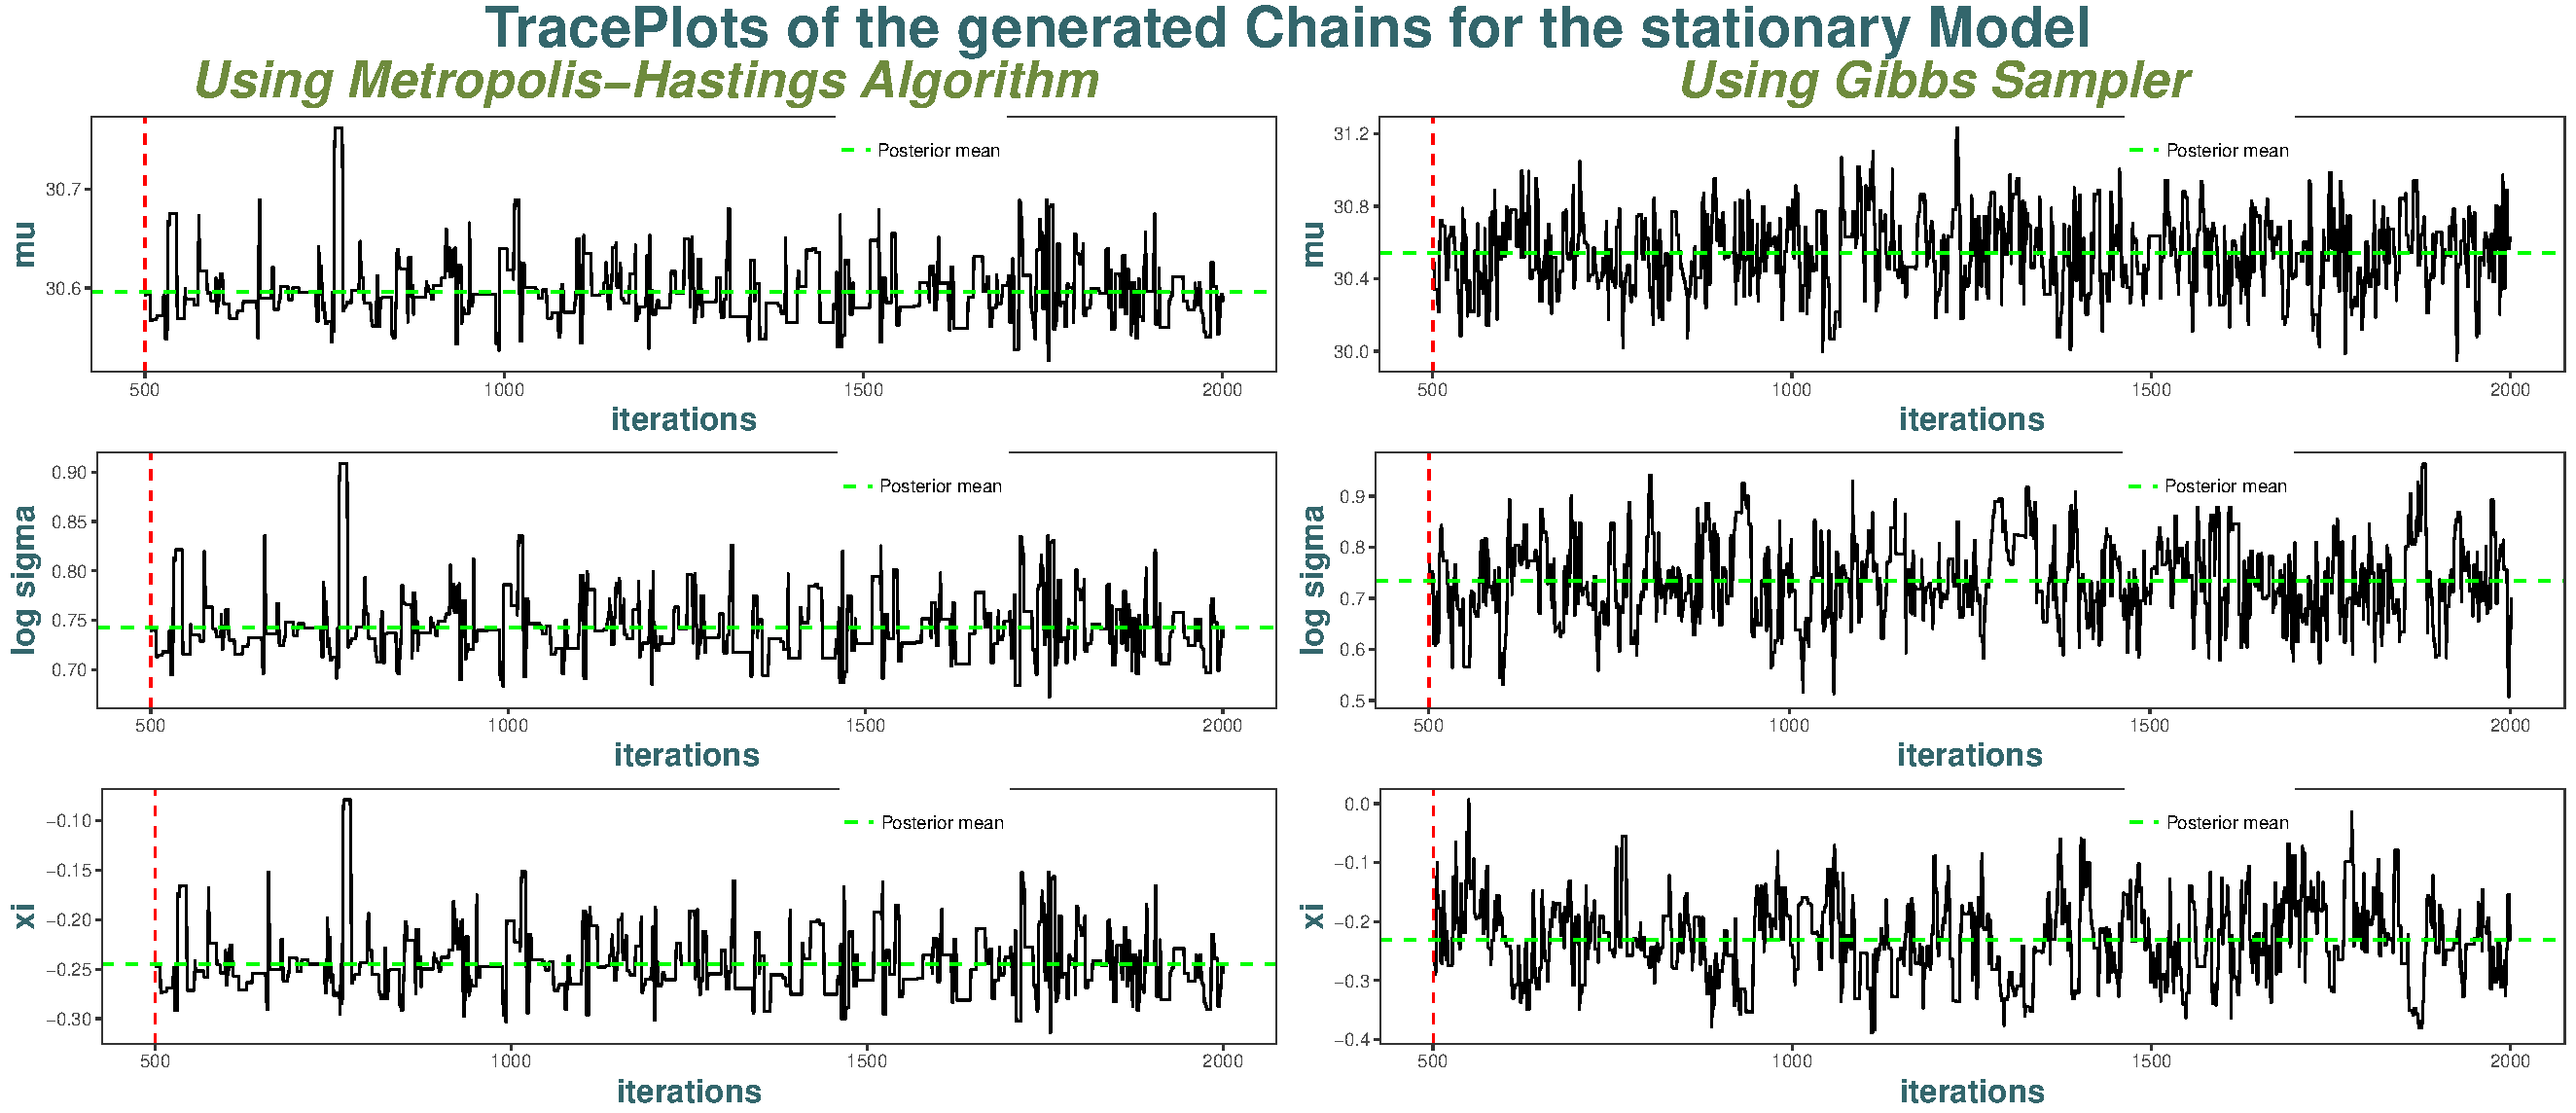
\includegraphics[width=5cm]{mhgib.pdf} } } \\
	
	\subfloat[fig 2]{{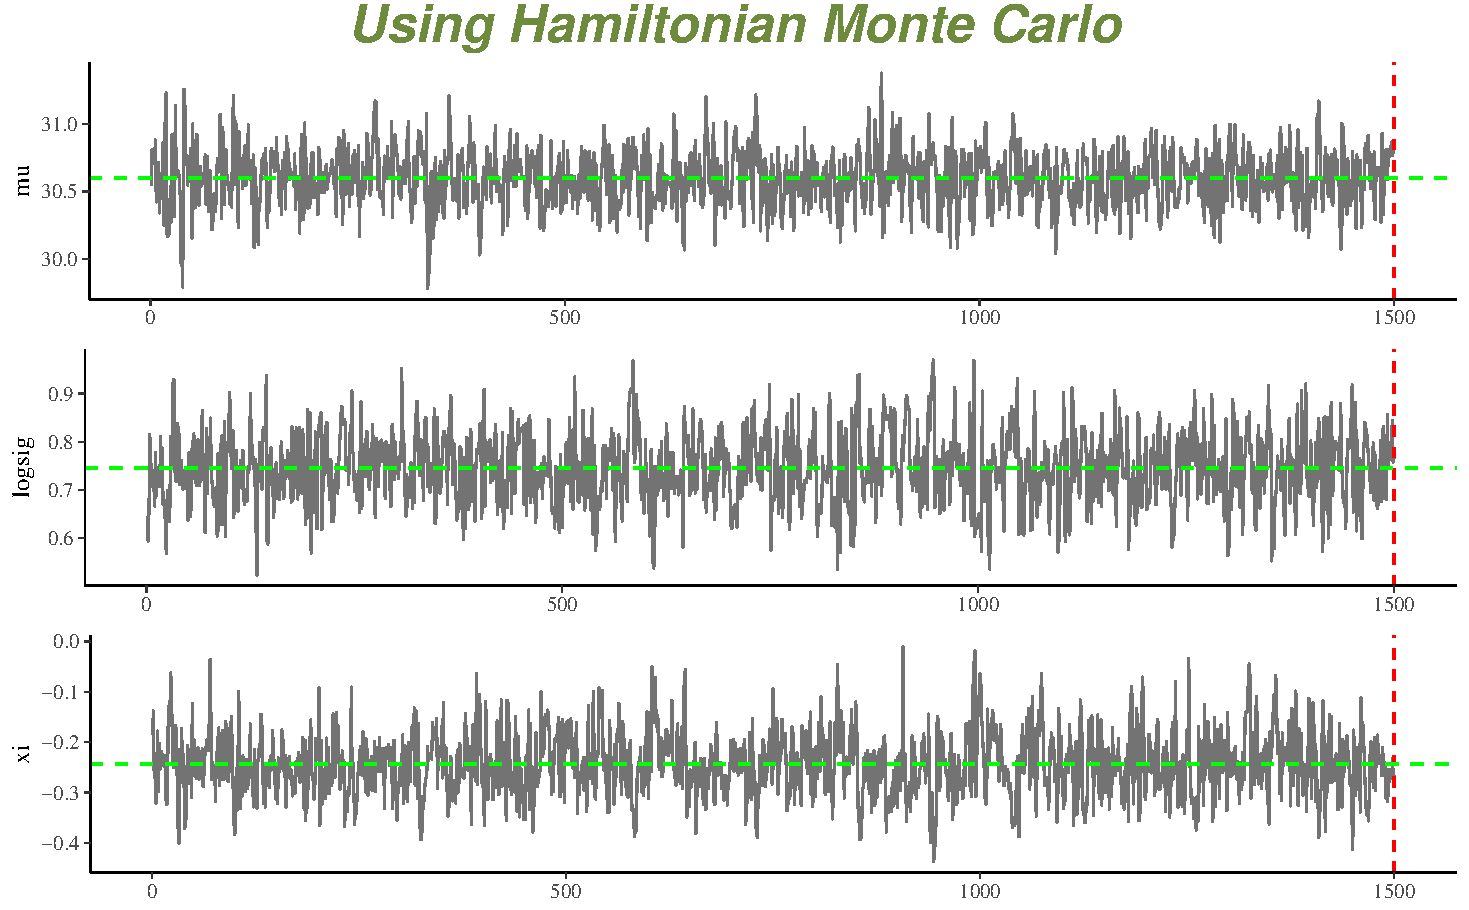
\includegraphics[width=5cm]{tracehmc.pdf} }}
	\caption{ Chains of the two usual Bayesian algorithms. Acceptance rate is $\approx0.21$ of the MH and individual acceptances rates all between $0.42$ and $0.50$ for the Gibbs sampler. We ran one single chain for both algorithms with the same starting values.}\label{fig:mhgibbs}
\end{figure}
\fi 

\begin{figure}[!htb]
	\centering	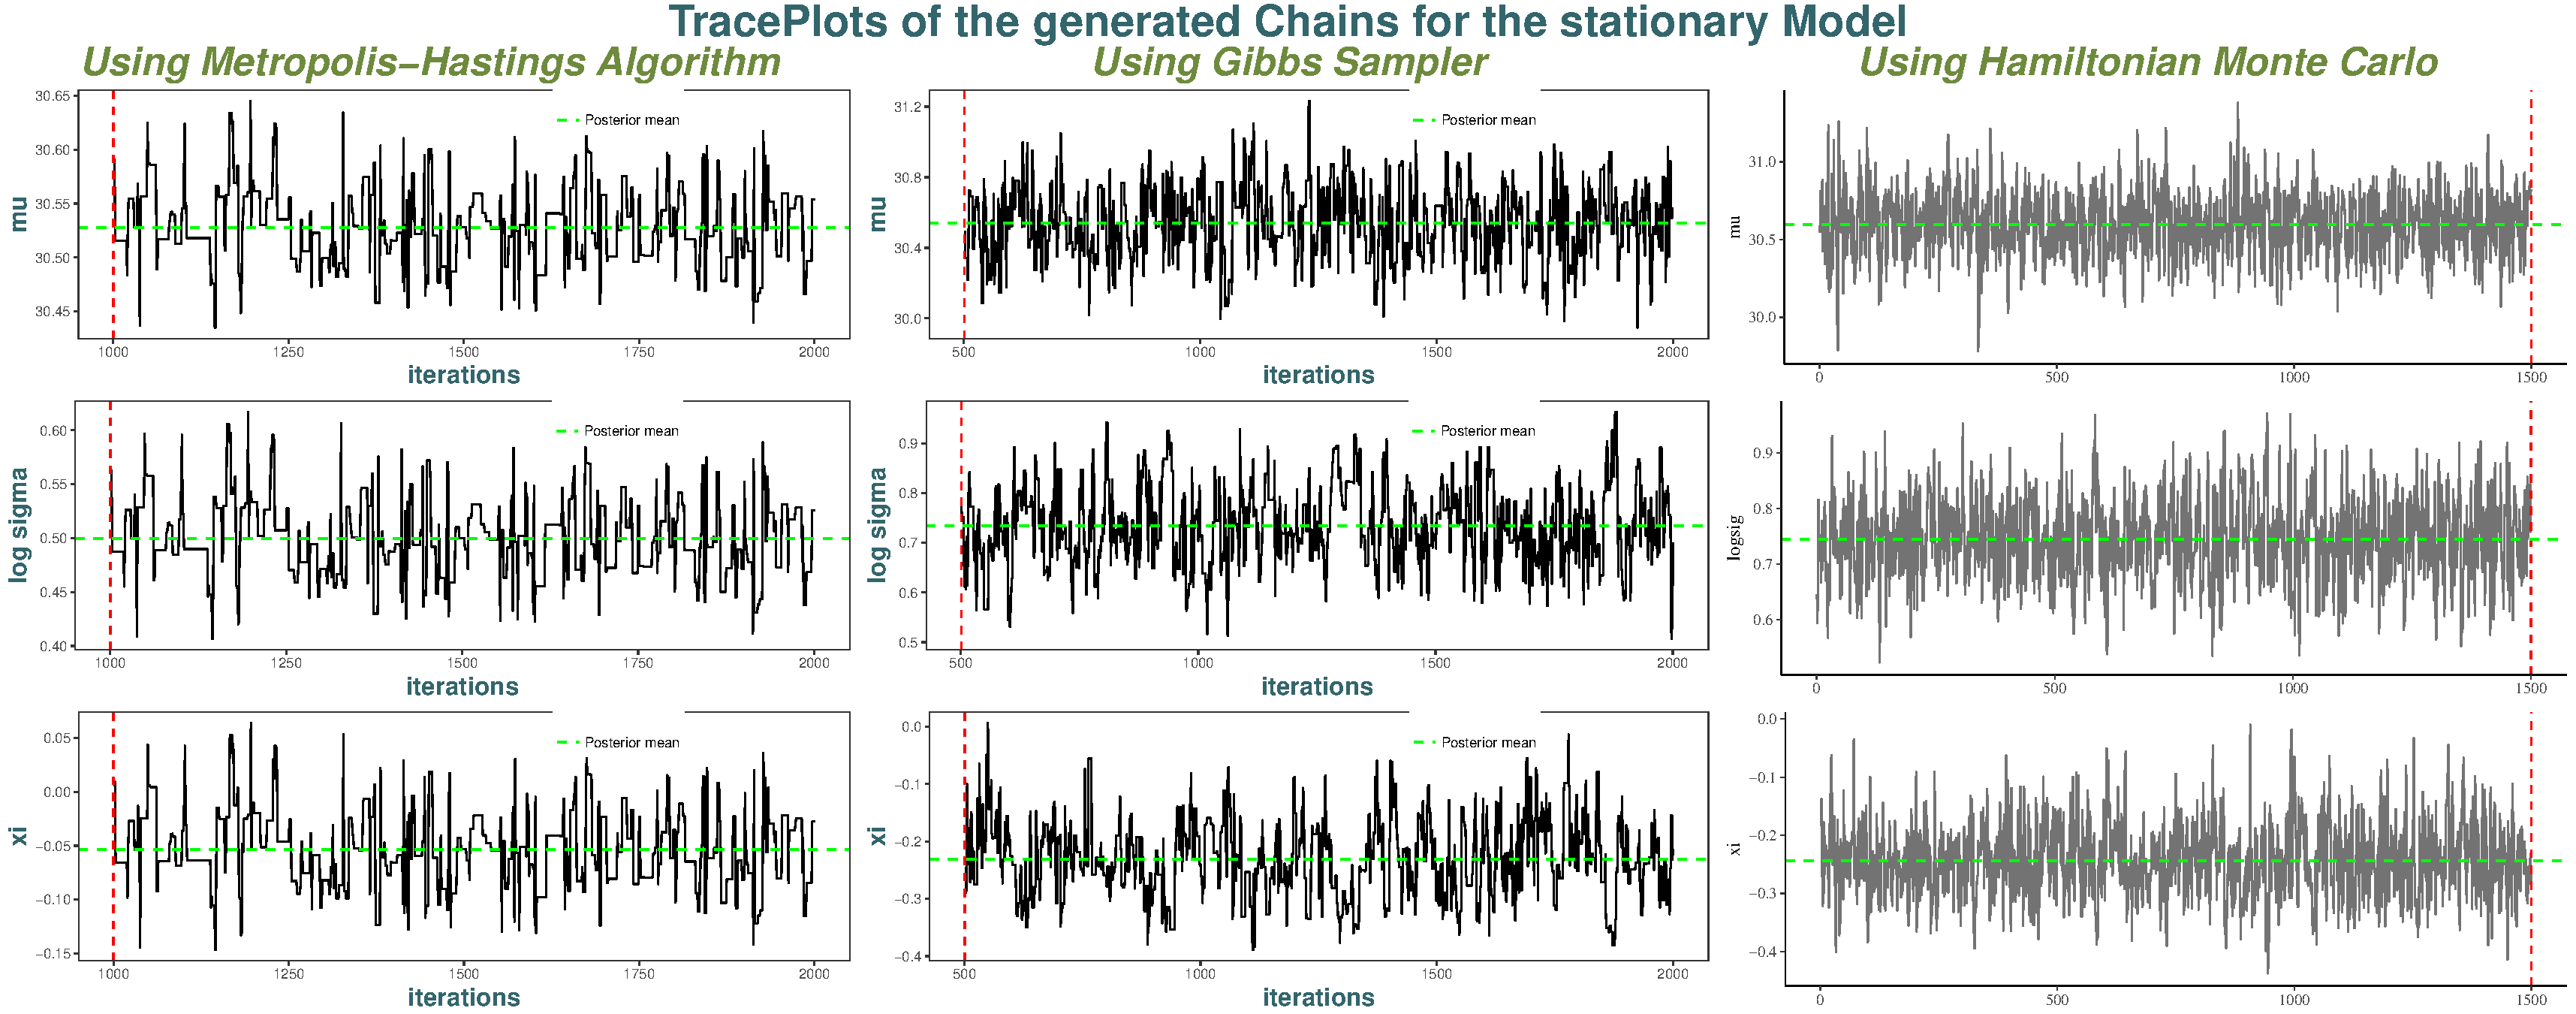
\includegraphics[width=1\linewidth]{traceall.pdf}	\caption{ Traceplots of the single chains chains generated by the three usual Bayesian algorithms considered. Acceptance rate is $\approx0.21$ of the MH and individual acceptances rates all between $42\%$ and $50\%$ for the Gibbs sampler. In the HMC, $49$ iterations are divergent and the acceptance rate statistic is of  $94\%$.
	We ran one single chain for all algorithms with the same starting values.}\label{fig:mhgibhmc}
\end{figure}


\begin{figure}[!htb]
	\centering	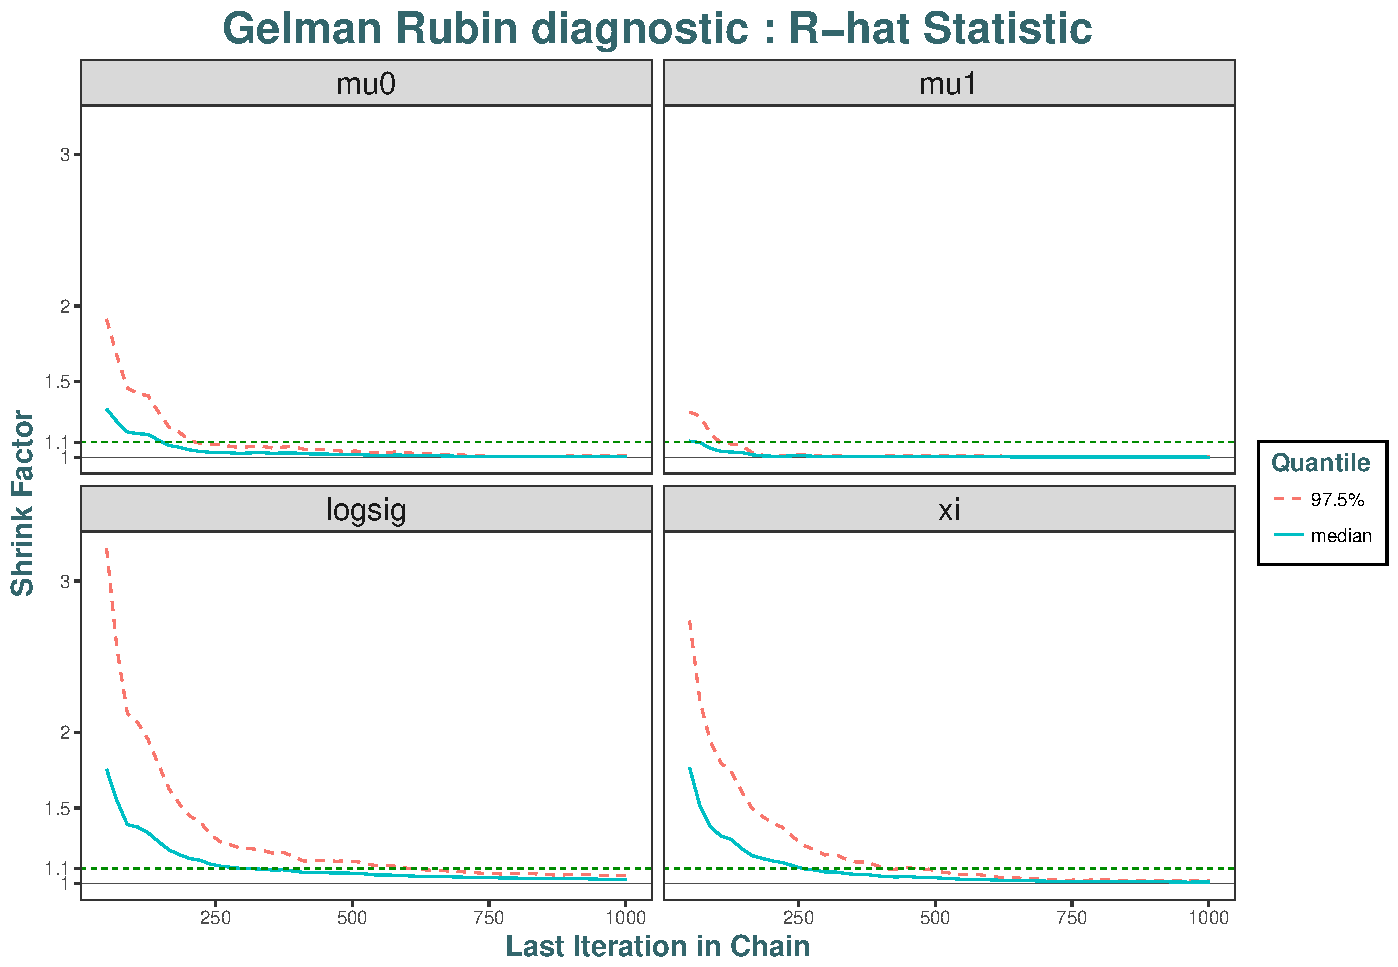
\includegraphics[width=0.7\linewidth]{gelmdiag.pdf}\caption{Gelman-Rubin diagnostic : $\hat{R}$ statistic computed by each repeating blocks of iterations, for each parameters. We refined the basic plot provided by \texttt{coda} in order to put the four graphs on the same $y$-scale, for comparison purposes.}\label{fig:gelmdiag}
\end{figure}


\begin{figure}[!htb]
	\centering	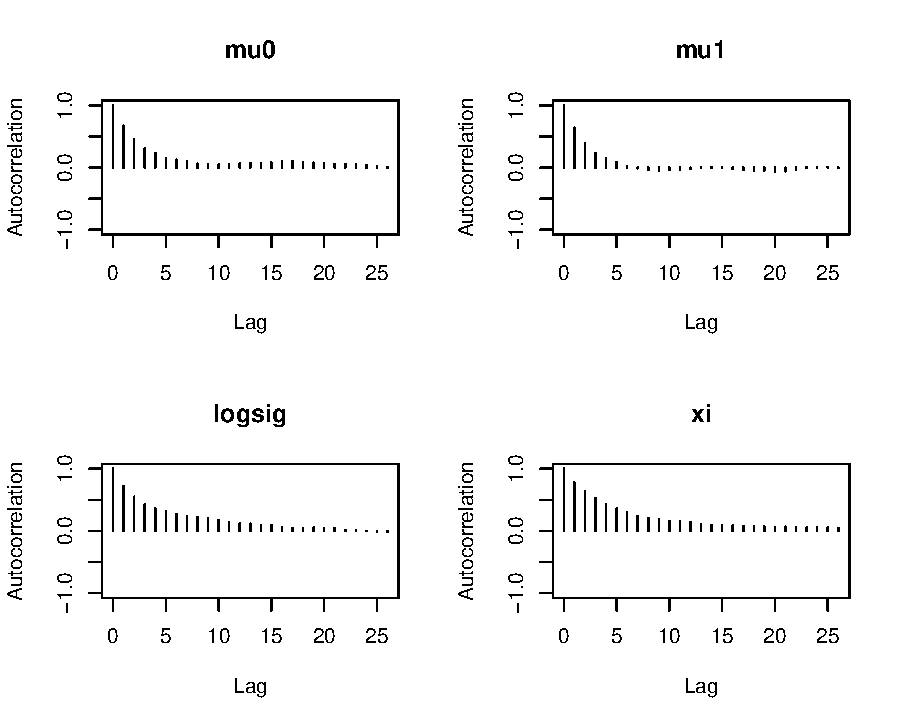
\includegraphics[width=0.8\linewidth]{autocor.pdf}\caption{Autocorrelation functions for each of the parameters' Markov chains for a maximum lag of 25. Output provided by \texttt{coda}. }\label{fig:autocor}
\end{figure}

\begin{figure}[!htb]
	\centering	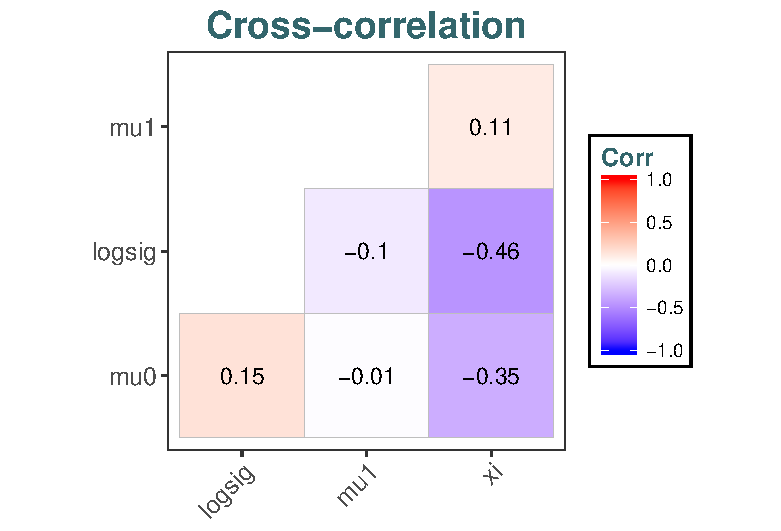
\includegraphics[width=0.5\linewidth]{crosscorr.pdf}\caption{Cross-correlation between each of the parameters' Markov chains.}\label{fig:crosscorr}
\end{figure}


\begin{figure}[!htb]
	\centering	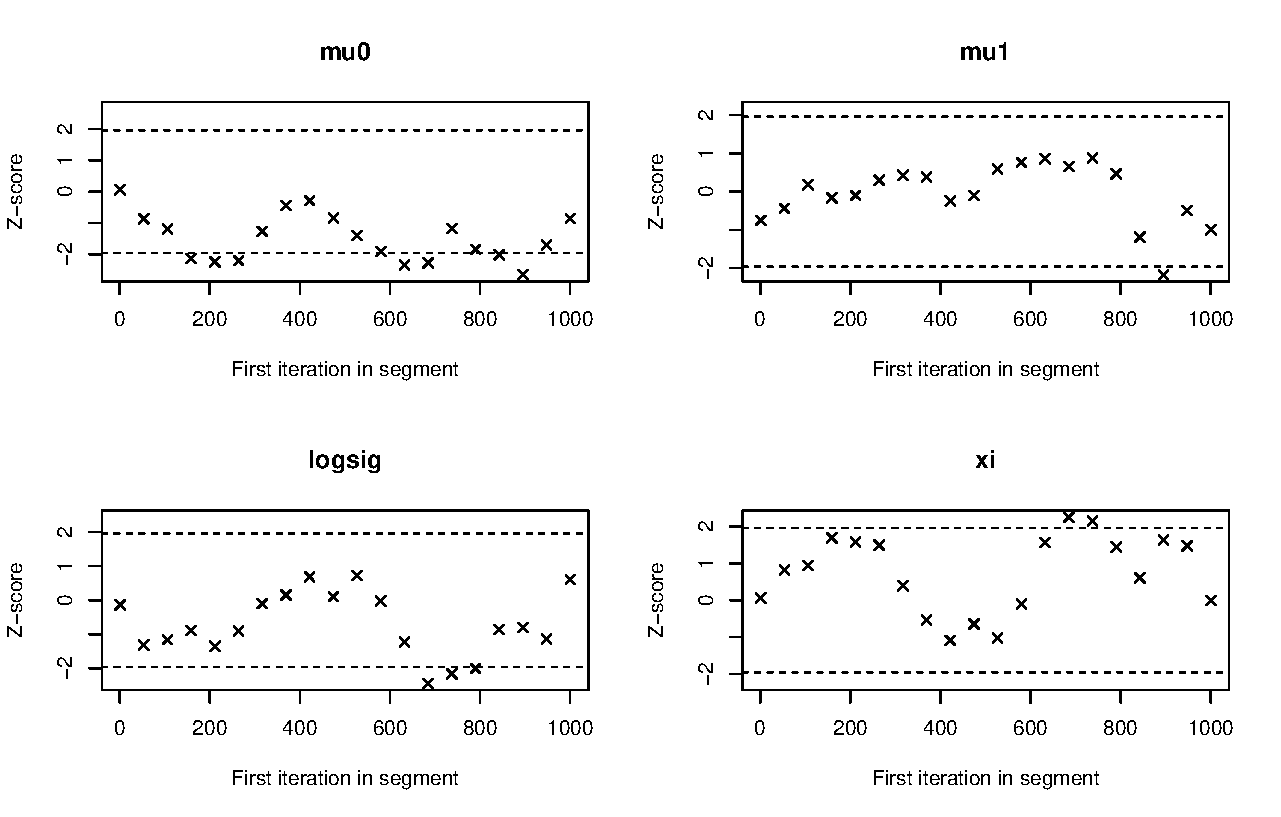
\includegraphics[width=0.7\linewidth]{geweke.pdf}\caption{Geweke diagnostic : compute $20$ z-scores that test the equality of the means between $10\%$ and $50\%$ of the chains. Dotted horizontal lines indicates the confidence regions at $95\%$. }\label{fig:geweke}
\end{figure}


\begin{table}[!htb] \centering 
	\begin{tabular}{@{\extracolsep{5pt}} c|cccc} 
\toprule
		& $B$ & $N_{\text{advised}}$ & $N_{\text{min}}$ & Dependence Factor \\ 
\midrule
$\mu_0$ & $17$ & $2189$ & $457$ & $4.790$ \\ 
$\mu_1$ & $13$ & $1689$ & $457$ & $3.700$ \\ 
$\log\sigma$ & $12$ & $1573$ & $457$ & $3.440$ \\ 
$\xi$ & $16$ & $2110$ & $457$ & $4.620$ \\ 
\bottomrule
	\end{tabular} 
		\caption{Raftery-Lewis diagnostic. "$B$" is the avdised number of iterations to be discarded at the beginning of each chain. "$N_{\text{advised}}$ " is the advised number of iterations. 
			 "$N_{\text{min}}$" is the minimum sample size based on zero autocorrelation. 
			 The "dependence factor" informs to which extent the autocorrelation in the chains inflates the required sample size, with values above 5 indicating a strong autocorrelation.  } 
		\label{tab:raf} 
\end{table} 


\chapter{Other Figures and Tables}\label{app:fig}

%\section{GEV : Influence of the Parameters on the Shape of the Distribution}

Regarding our future application, that is maximum temperatures, it is relevant to consider values of the location parameter $\mu$ around 30 degrees. 


\begin{figure}[!htb]
	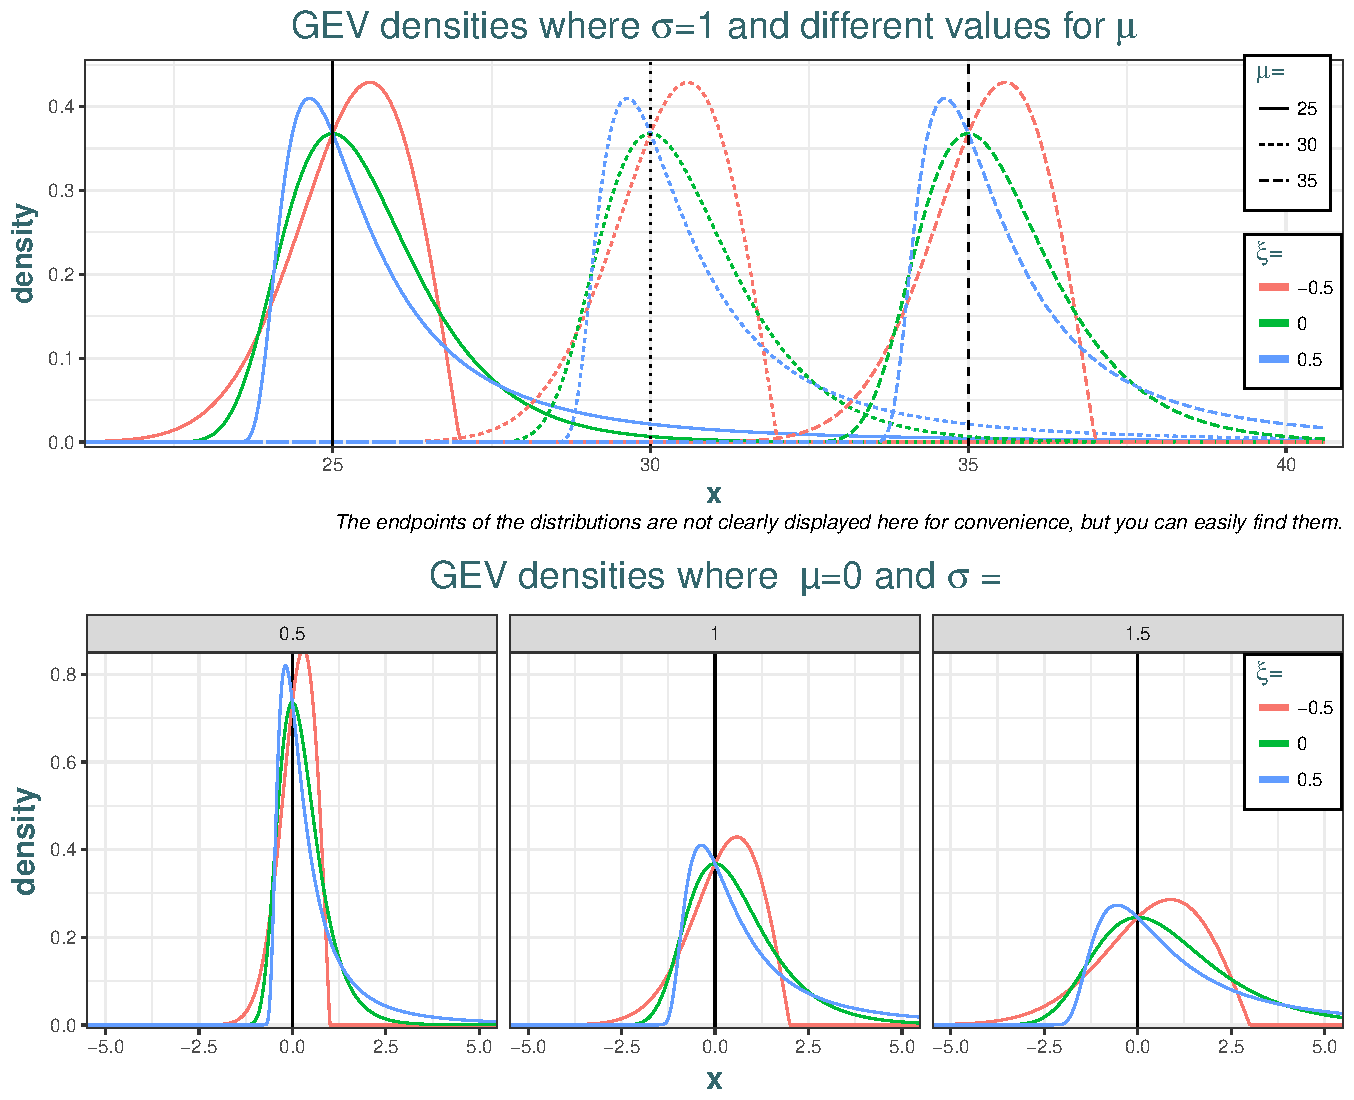
\includegraphics[width=\linewidth]{gevdif.pdf}\caption{GEV distribution for different values of the three parameters }\label{fig:gevdif}
\end{figure}


%\section{Introduction of the Practical Analysis (section 6)}


\begin{figure}[!htb]
	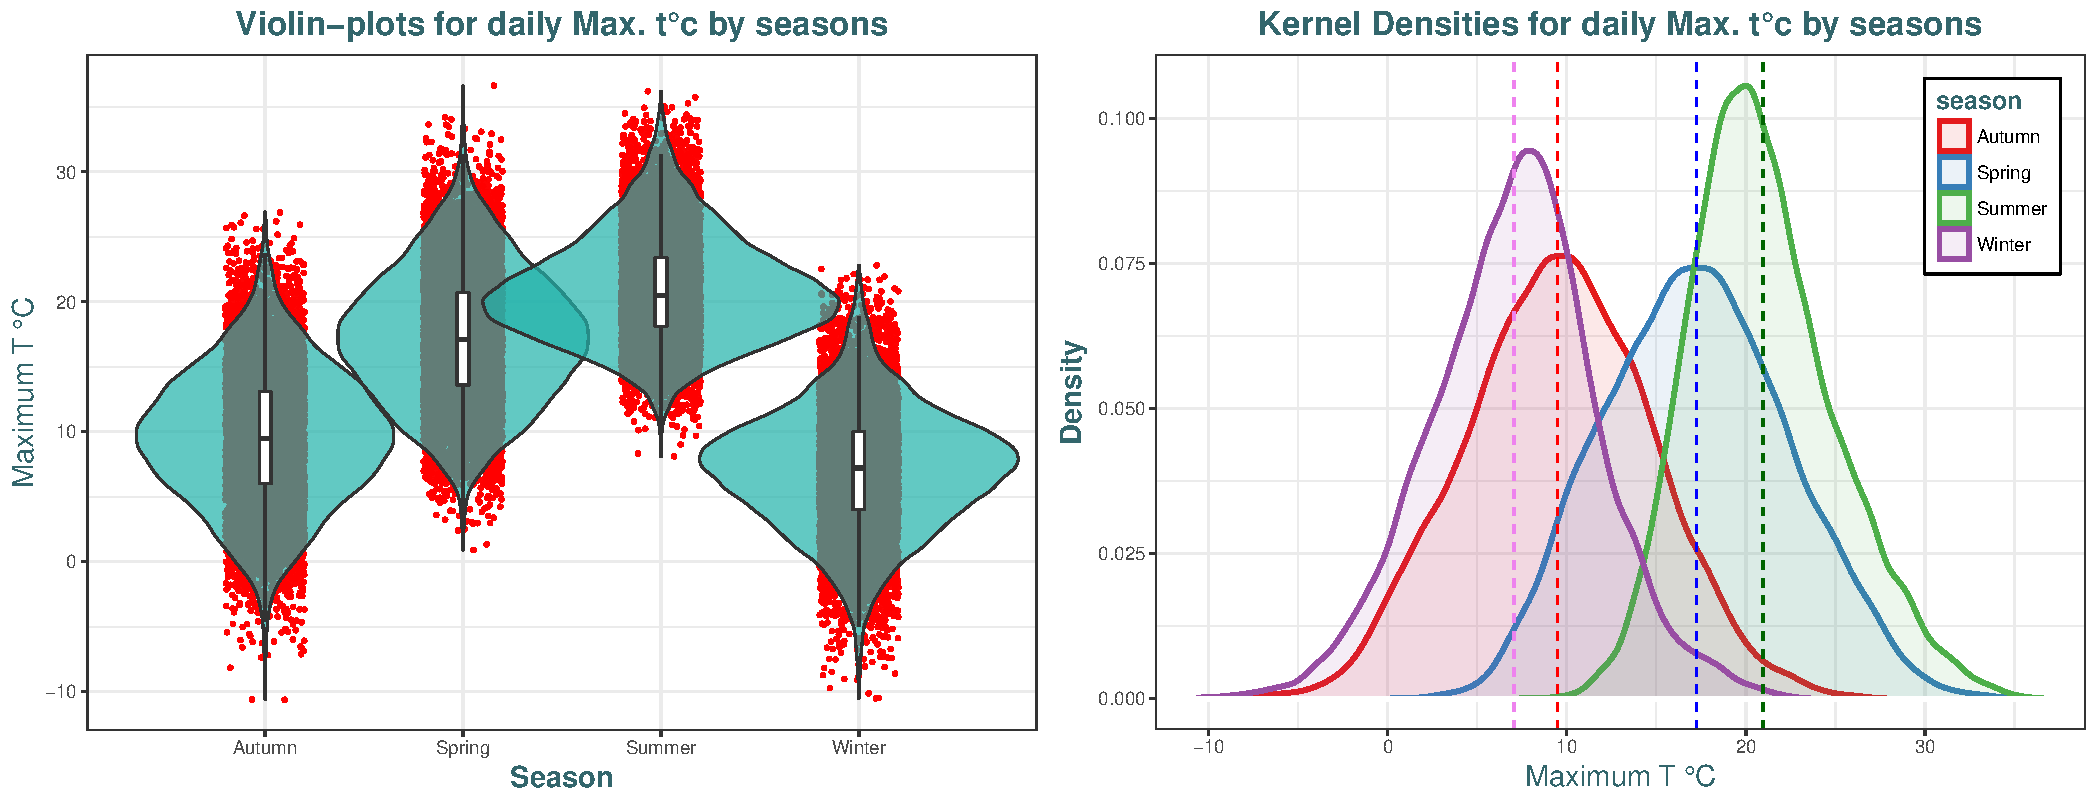
\includegraphics[width=1\linewidth]{violin_density.pdf}\caption{ Violin-plot (left) and density plots (right) for each seasons. In the density plots, vertical dotted lines represent the mean of each distribution.}\label{fig:violin_density}
\end{figure}

\begin{figure}[!htb]
	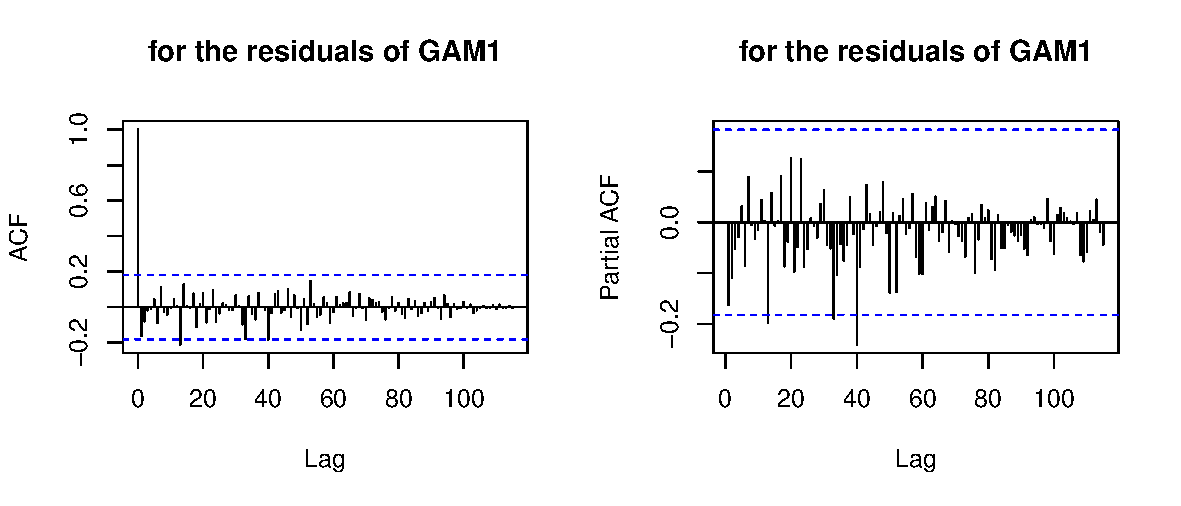
\includegraphics[width=\linewidth]{acfresgam.pdf}\caption{ACF and PACF for the residuals of the fitted GAM model with assumed independent errors }\label{fig:acfresgam1}
\end{figure}

\begin{table}[!htbp] \centering 
  \caption{Models' comparisons for the residuals of the GAM model based on AIC and BIC criterion. } 
  \label{table:gamresid} 
\begin{tabular}{@{\extracolsep{5pt}} ccccc} 
\\[-1.8ex]\hline 
\hline \\[-1.8ex] 
& df & AIC & BIC \\ 
\hline \\[-1.8ex] 
Uncorrelated  & $4$ & $494.635$ & $505.650$ \\ 
AR(1)  & $5$ & $494.356$ & $508.124$ \\ 
MA(1) & $5$ & $493.706$ & $507.474$ \\ 
ARMA(1,1)  & $6$ & $492.511$ & $509.033$ \\ 
AR(2)  & $6$ & $495.133$ & $511.654$ \\ 
MA(2)  & $6$ & $494.698$ & $511.219$ \\ 
\hline \\[-1.8ex] 
\end{tabular} 
\end{table}


\begin{figure}[!htb]
\centering	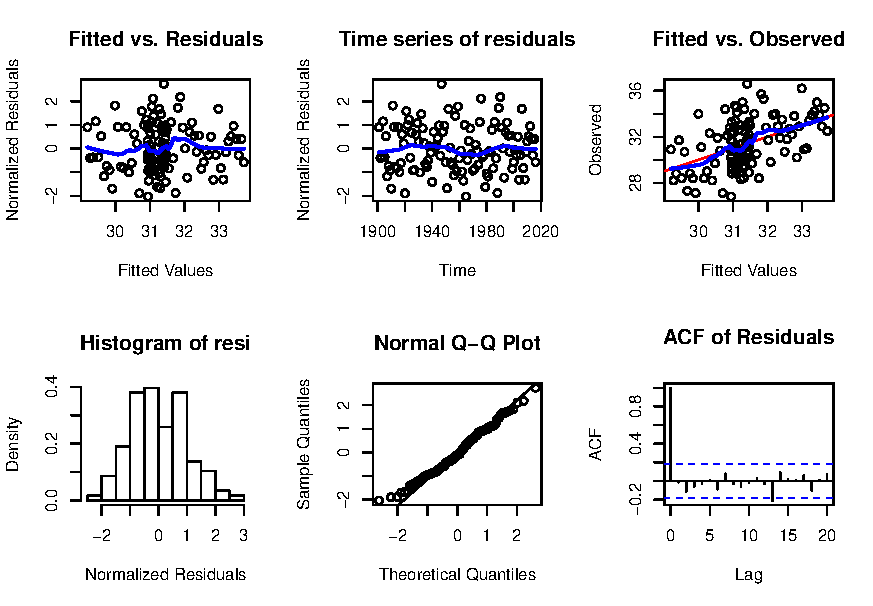
\includegraphics[width=.85\linewidth]{diagnogam.pdf}\caption{Diagnostics of the chosen GAM model with Whinte Noise process on the errors, based on the residuals. }\label{fig:diagnogam}
\end{figure}


\begin{figure}[!htb]
\centering	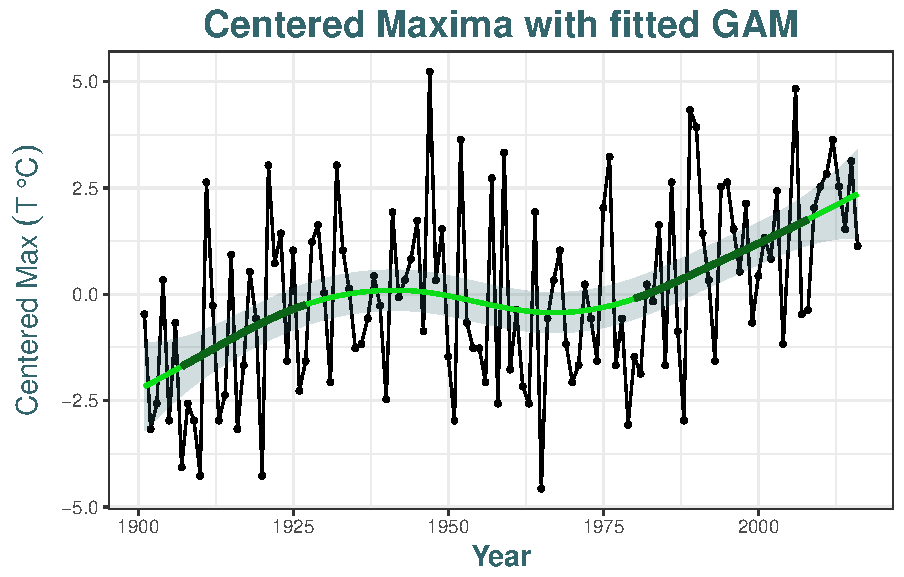
\includegraphics[width=.7\linewidth]{max_gam.pdf}\caption{Series of annual maxima together with the fitted GAM model (in green) \textbf{with MA(1) model on the residuals}. Thicker lines indicate that the increase is significant for \underline{pointwise} confidence interval. Shaded area represent a "$95\%$" interval for the predicted values which looks quite narrow. }\label{fig:center_gam}
\end{figure}




%\section{Analysis by GEV}


\begin{figure}[!htb]
\centering	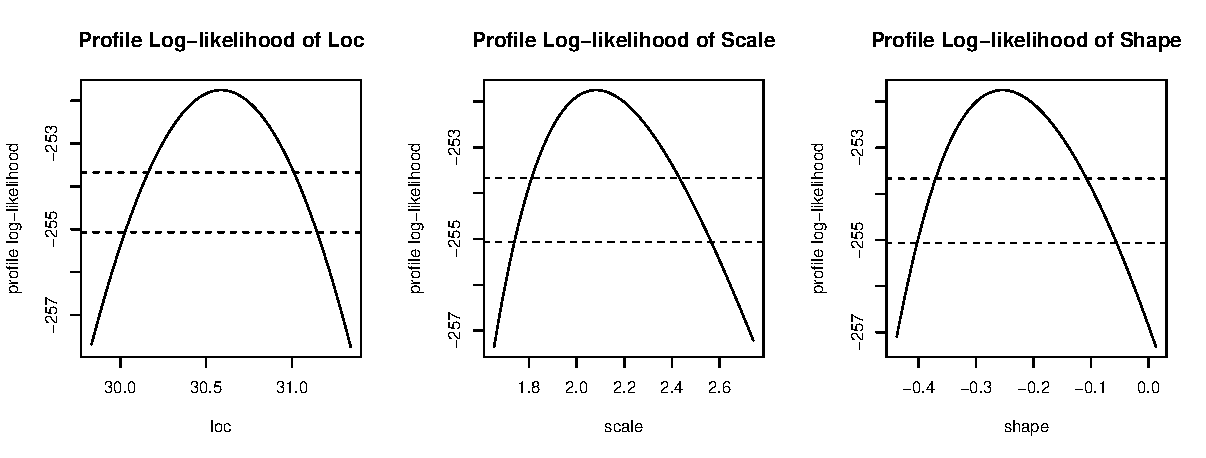
\includegraphics[width=.85\linewidth]{proflikpar.pdf}\caption{ Profile likelihood intervals for the stationary GEV parameters. The two horizontal dotted lines represent the 95$\%$ (above) and $99\%$ (below) confidence intervals by taking the intersection with the horizontal axis.}\label{fig:proflikpar}
\end{figure}



\begin{figure}[!htb]
	\centering	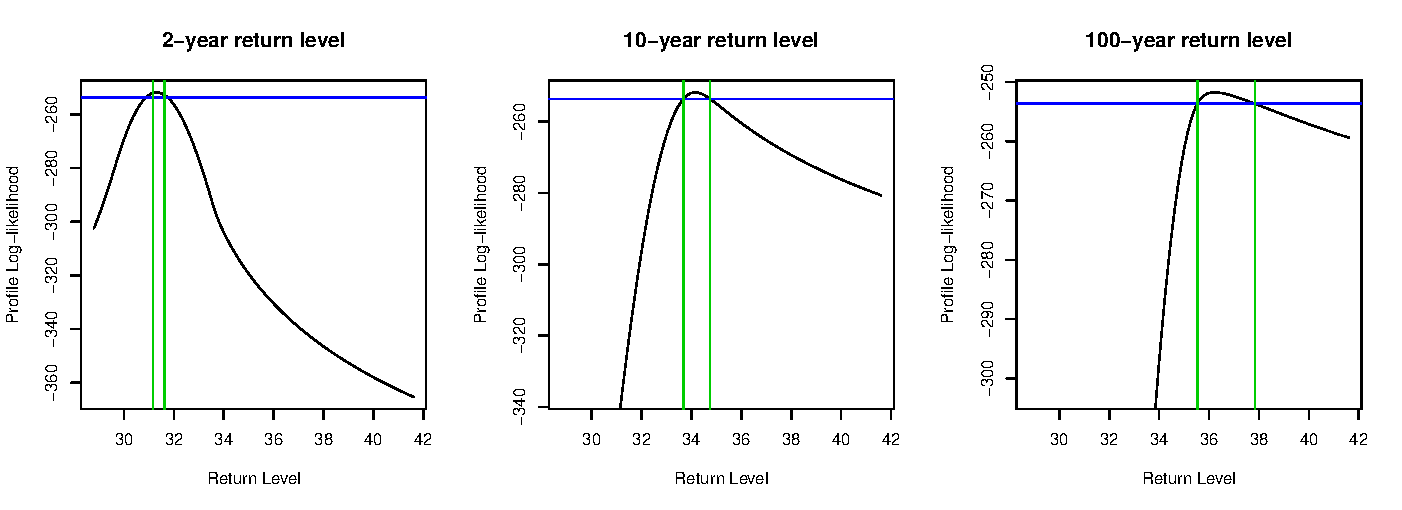
\includegraphics[width=.95\linewidth]{proflikrl.pdf}\caption{ $95\%$ Profile likelihood intervals for return levels with return periods of $2$, $10$ and $100$. We kept the same $x$-scales for the three plots but not the $y$-scales. We used the \texttt{ismev} package but we modified the function to allow for more flexibility because the default y-scale in produced ugly visualizations for high return levels. Green lines represent the intervals from Table \ref{tab:rl1} computed with another package from E.Gilleland, \texttt{extRemes}. }\label{fig:proflikrl}
\end{figure}


\begin{figure}[!htb]
	\centering	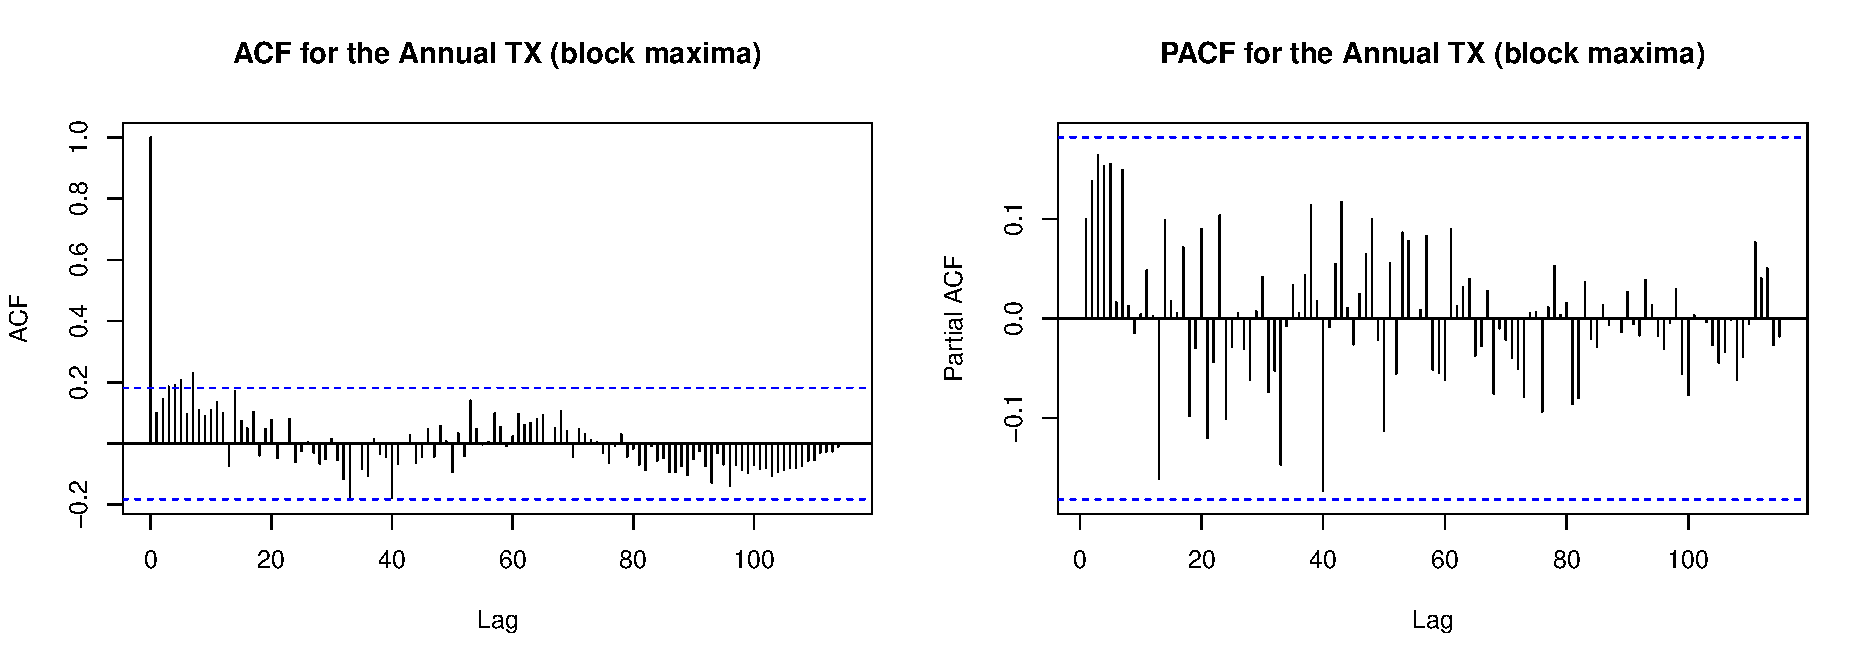
\includegraphics[width=.95\linewidth]{acf_gev.pdf}\caption{Autocorrelation functions for the series of annual maxima.}\label{fig:acf_gev}
\end{figure}




\begin{figure}[!htb]
\centering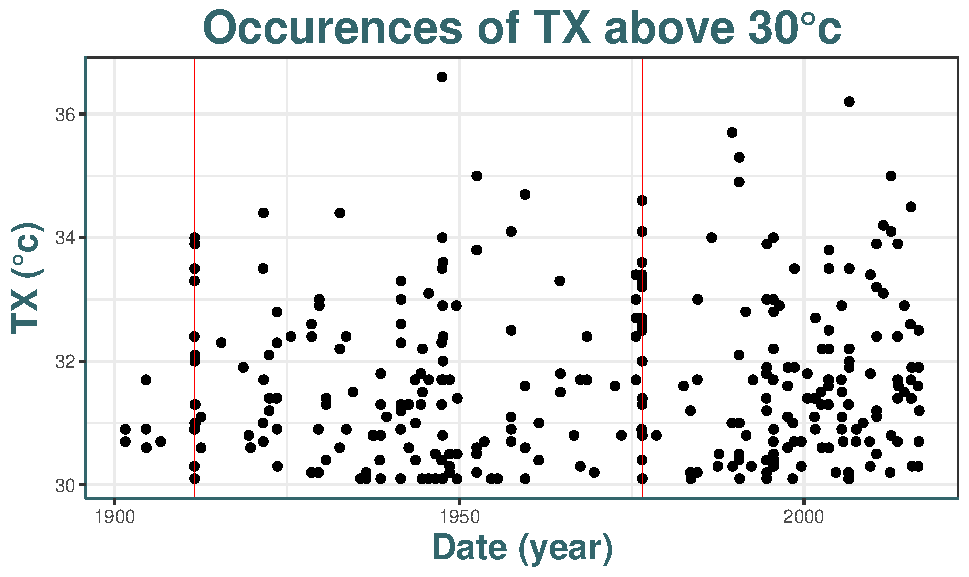
\includegraphics[width=0.7\linewidth]{abo.pdf}
\caption{Plot of all daily TX that exceeded $30^{\circ}c$ in the period [1901,2016] in Uccle. Red lines highlights two periods of heavy heat waves during summers 1911 and 1976.}\label{fig:abo}
\end{figure}


 \begin{table}[!htbp]
 	\centering 
 	\begin{tabular}{@{\extracolsep{5pt}} cccccc} 
 		\toprule
 		& Location $\beta_0$ & Location $\beta_1$ & Scale $\alpha_0$ & Scale $\alpha_1$ &  Shape $\xi$ \\ 
 		\midrule
 		Estimates& $\textcolor{red}{29.19}$& $\textcolor{red}{0.0242}$ & $\textcolor{red}{0.686}$  &  $\textcolor{red}{-0.0012}$ & $-0.199$ \\ 
 		\bottomrule
 	\end{tabular} 
 	 	\caption{Estimation of the bootstrap aggregated GEV-CDN model with 2 hidden layers for $\sigma(t)$ and $\mu(t)$, and $M=500$ resamples. In red are denoted rough estimates of the nonstationary parameters as if the model were parametric for both parameters $\sigma(t)= \exp (\alpha_0+\alpha_1\cdot t)$ and $\mu(t)=\beta_0+\beta1\cdot t$. But this is actually not reliable since there are 2 hidden layers, and only the shape parameter can be reliably estimated.} 
 	 	\label{tab:estnnbag} 
 \end{table} 
 
 
  \begin{figure}[!htb]
  	\centering	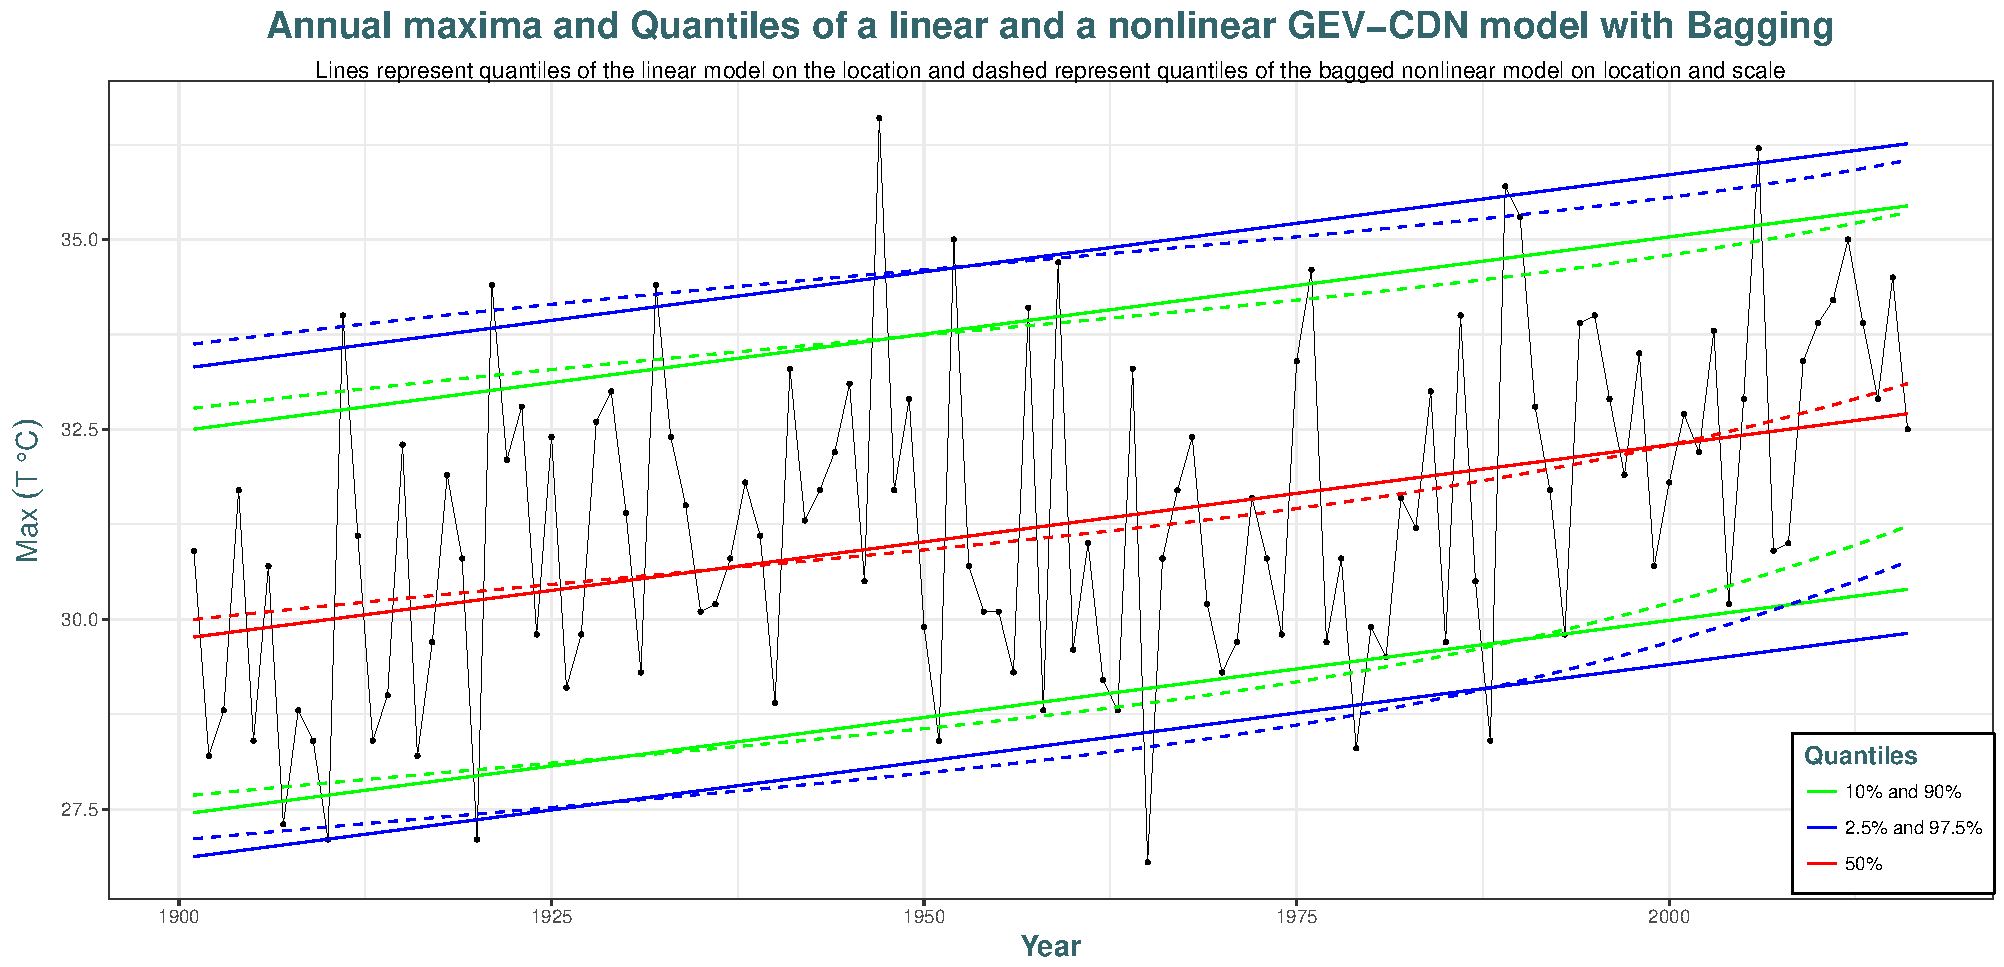
\includegraphics[width=0.9\linewidth]{gev_comp_v1.pdf}\caption{This graph gathers the two plots of Figure \ref{fig:bag} which could yield to a better visualization.  }\label{fig:bagv1}
  \end{figure}
  

  \begin{figure}[!htb]
  	\centering	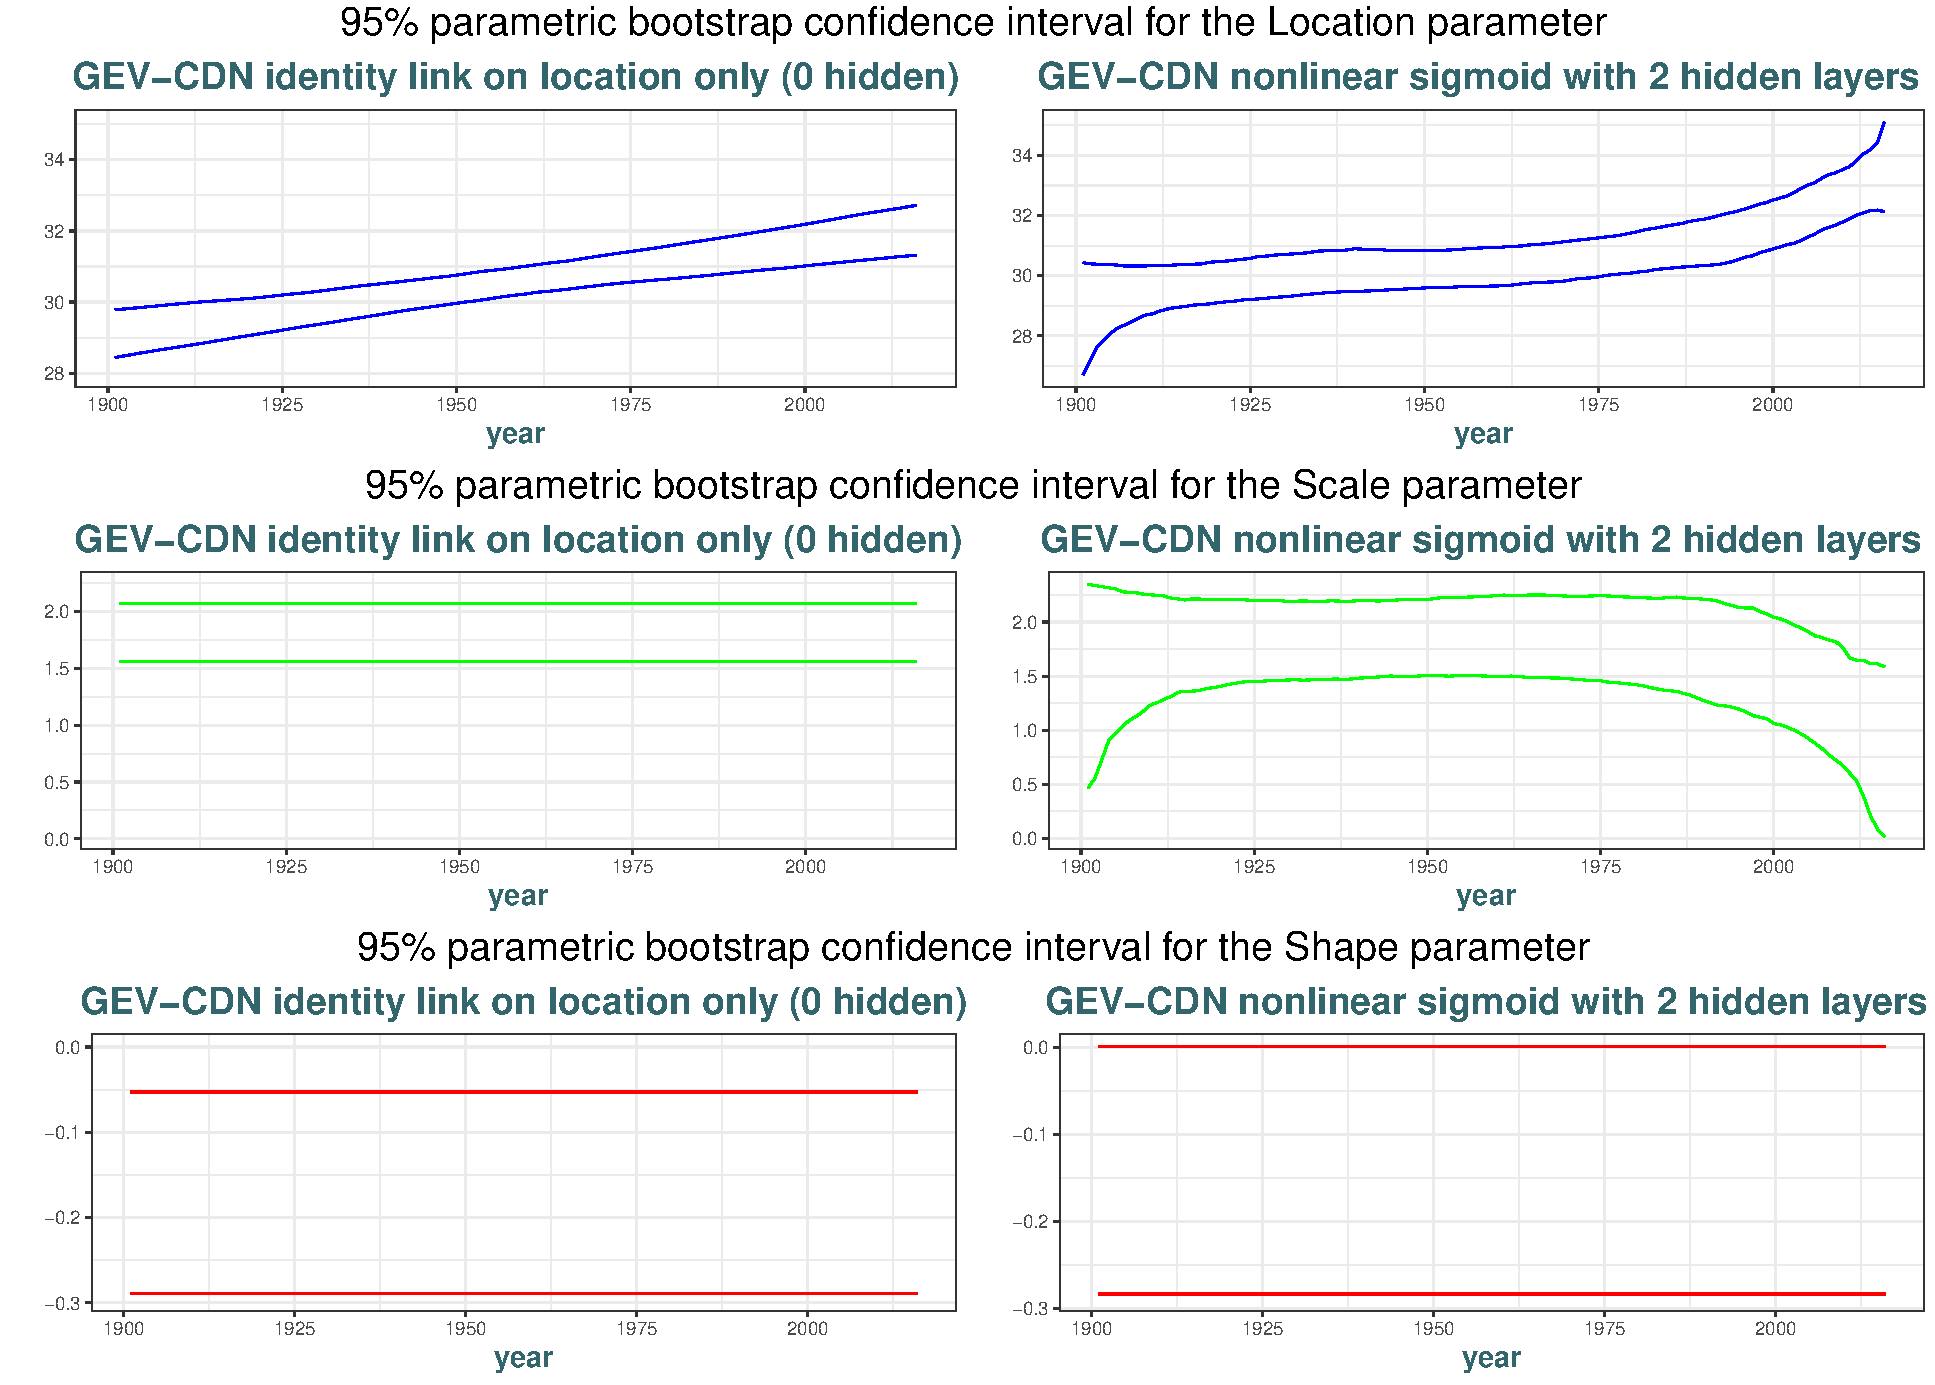
\includegraphics[width=1.01\linewidth]{g_boot_par.pdf}\caption{Left plots show the \textbf{parametric} bootstrap $95\%$ intervals computed with the GEV-CDN model allow a linear nonstationary location parameter only, and Right plots show these interval for the nonlinear nonstationary model in location and scale parameters with 2 hidden layes. }\label{fig:boot_par}
  \end{figure}


\iffalse
\begin{figure}
	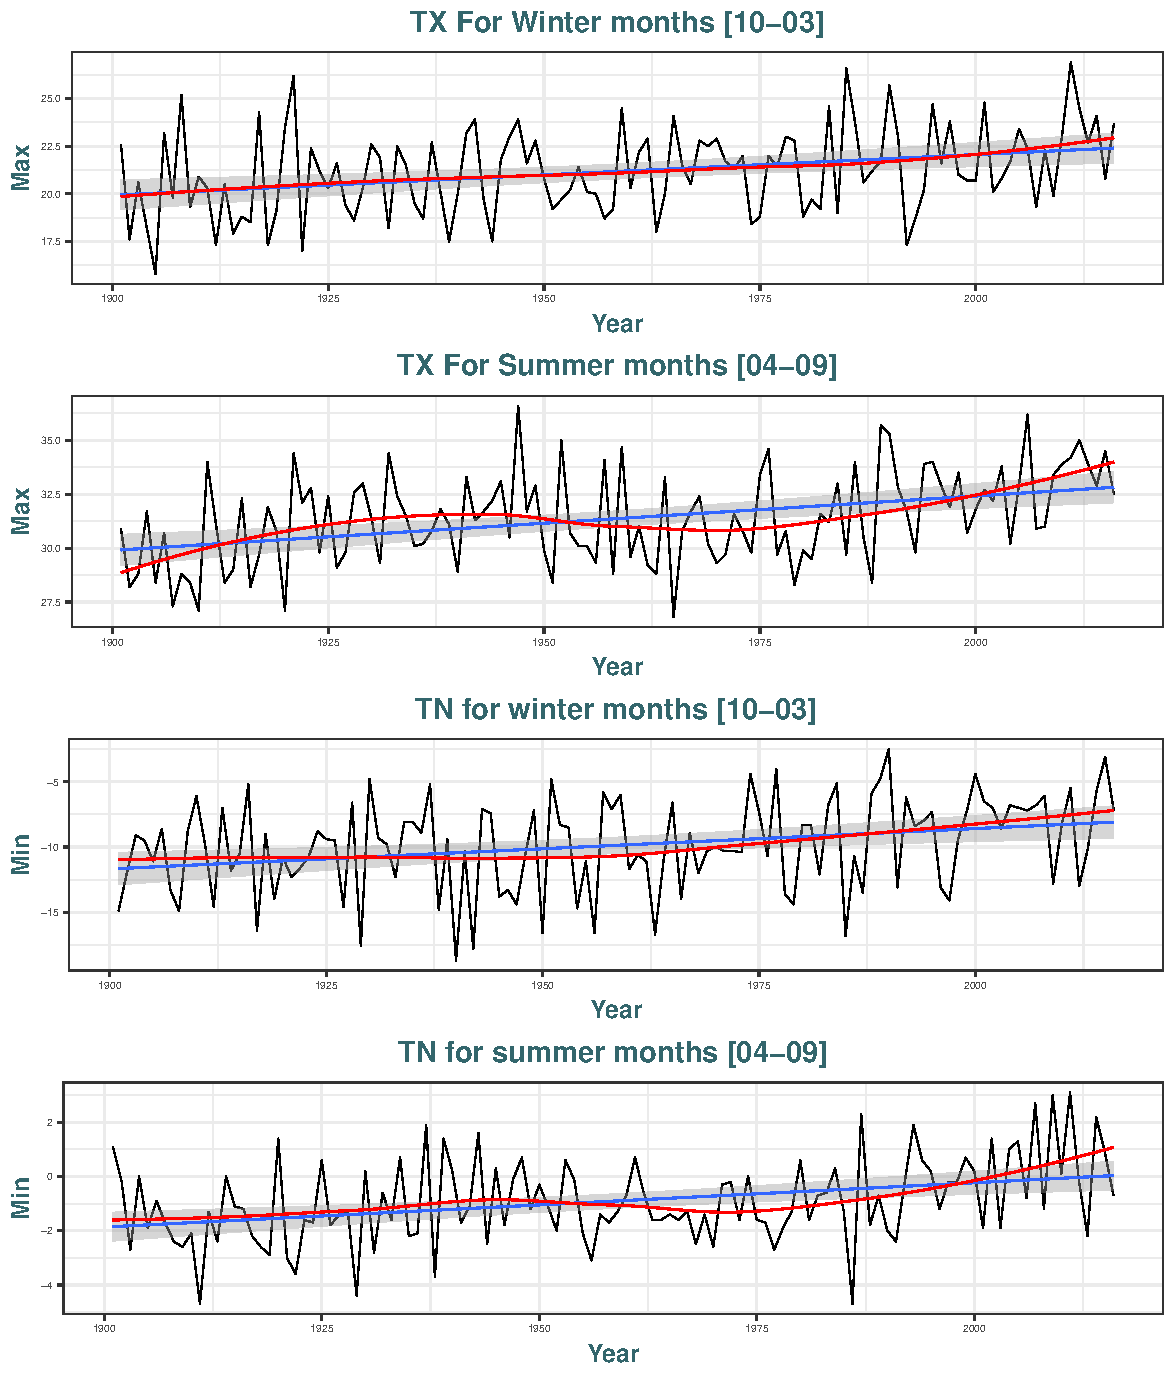
\includegraphics[width=.7\linewidth]{sumwint.pdf}\caption{First plot representing the \textbf{yearly} maxima (above) and minima (below) taking only the summer months (April to September) and winter months (October to March), shaded grey line around the linear trend represents its standard error. See how the polynomial trend (red line) also changes. Obv, TX for smummer and TN for winter are the same series as for the global serie}\label{seas4}
\end{figure}
\fi 


\iffalse
\begin{figure}[!h]
	\minipage{\textwidth}
	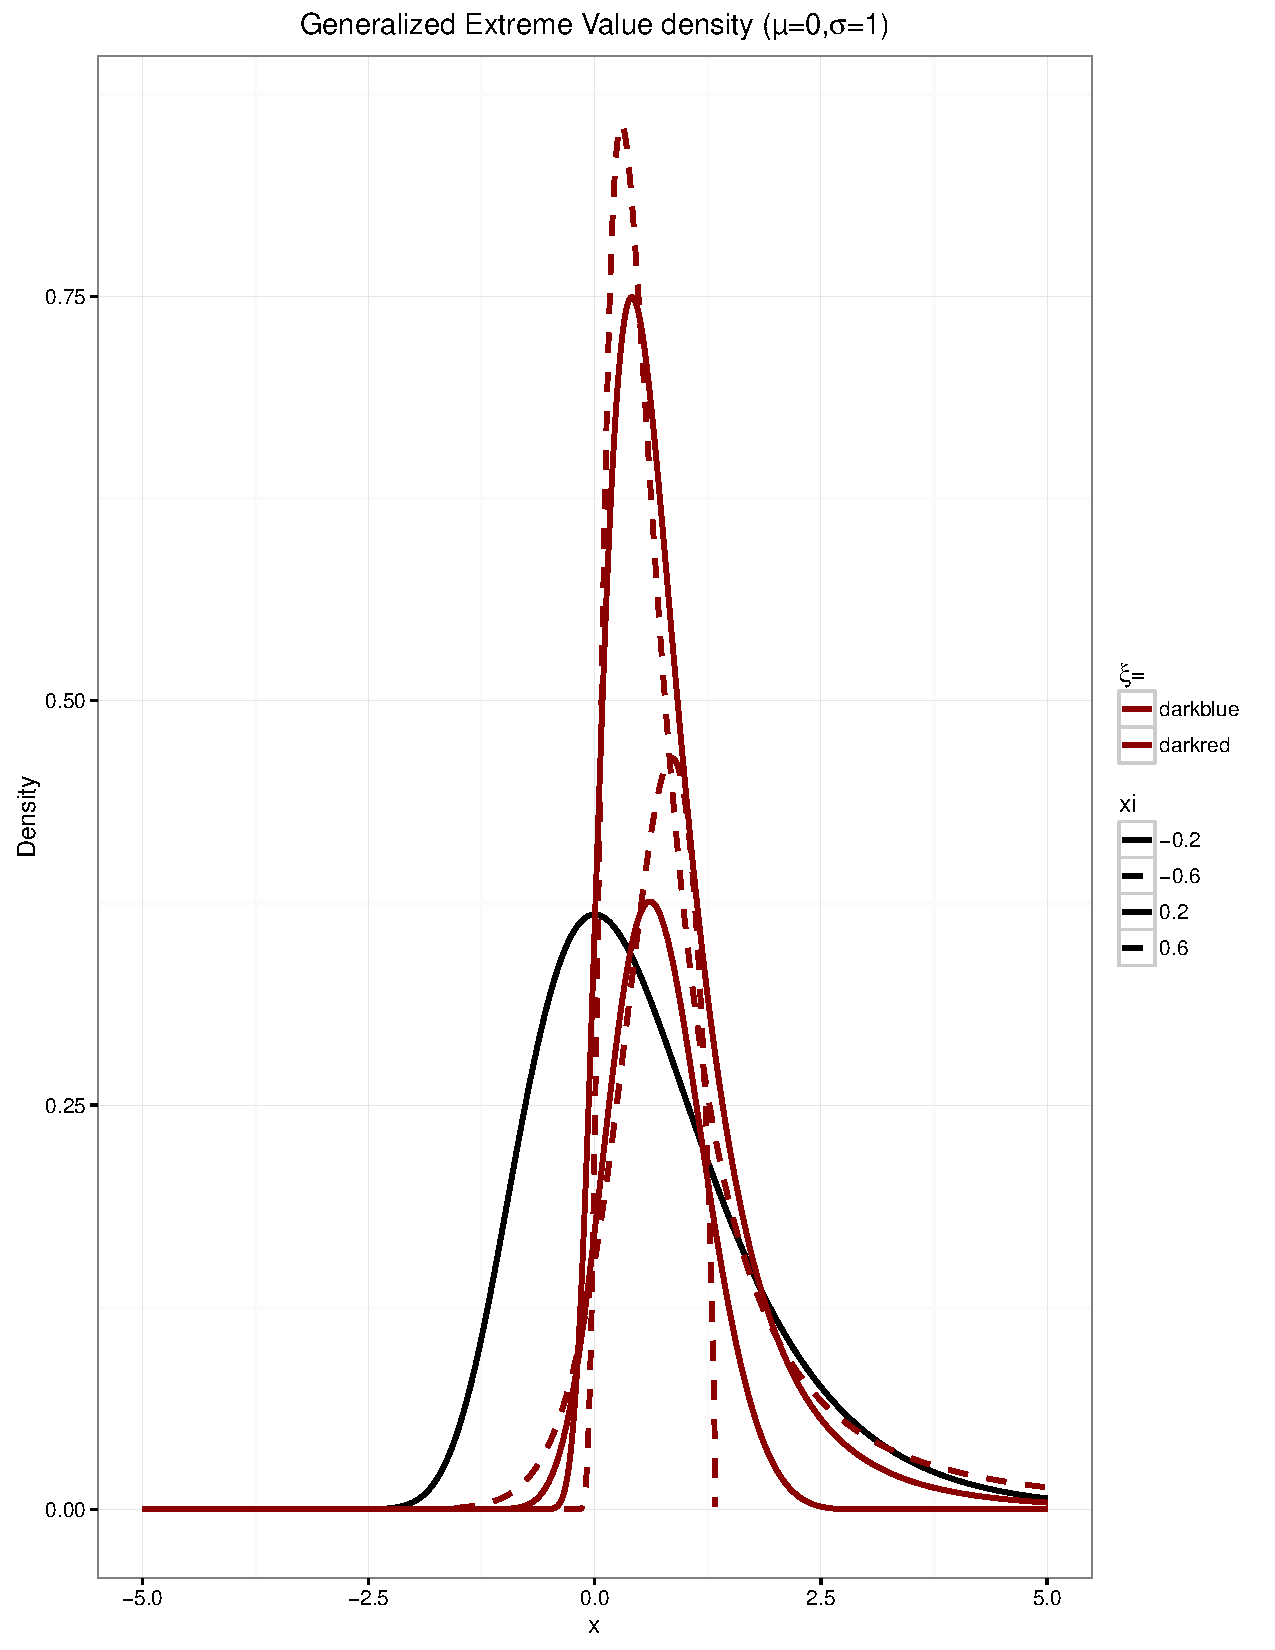
\includegraphics[width=\linewidth]{GEVV.pdf}
	\caption{ }\label{mcacls}
	\endminipage
\end{figure}
\begin{figure}[t!]
	$\begin{array}{rl}
	\multicolumn{2}{c}{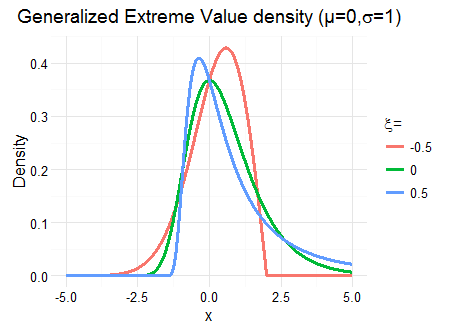
\includegraphics[width=0.85\textwidth]{GEV05.png}}\\
	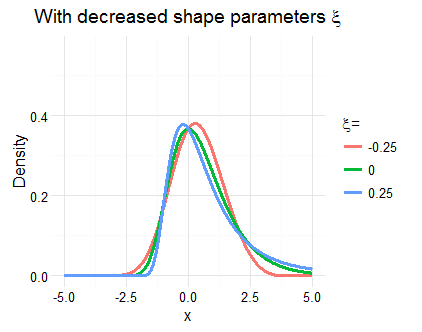
\includegraphics[width=0.5\textwidth]{GEV025.png} &
	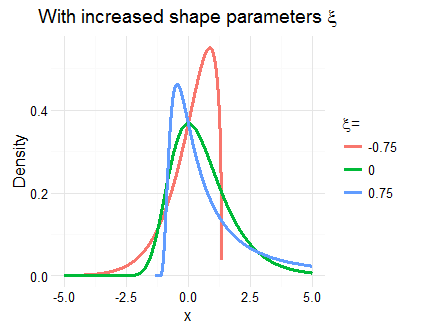
\includegraphics[width=0.5\textwidth]{GEV075.png}
	\end{array}$
	\caption{Representation of the GEV densities for various values of the shape parameter $\xi$ : $|\xi|=0.5$ (1) $|\xi|=0.25$, (2) and $|\xi|=0.75$ (3) for the Fréchet density [red], Weibull density [blue] while the Gumbel density [green] is kept fixed with $\xi=0$. }{\label{gevdens0}}
\end{figure}
\fi 


\chapter{Github Repository : Structure}\label{appgit}

From the huge amount of code needed for the analysis, we decided to divide it so that it will be more conveniently used and read. It was also preferred to create a R package to gather all the functions created.
The Github \href{https://github.com/proto4426/PissoortThesis/}{repository} build for this thesis can be found on this address :

\begin{center}
\url{https://github.com/proto4426/PissoortThesis}
\end{center}
where the R package \textbf{\texttt{PissoortThesis}} is located. The README file contains valuable information to install the package and provide an overview of the Shiny applications. It has the following structure, with \texttt{files} divided in \textbf{/folders/} : 

\begin{itemize}
\item \textbf{/R/} : Folder containing the scripts with all the functions that have been build for this thesis and are made available through the package. 

  \begin{itemize}
\item[$\vartriangleright$] \texttt{1UsedFunc.R} : functions created for the first part, including  the stationary analysis of annual maxima in GEV, analysis in POT, nonstationary analysis in GEV and POT, etc.
\item[$\vartriangleright$] \texttt{BayesFunc.R} : functions for the Bayesian Analysis, e.g. the Metropolis-Hastings and Gibbs Sampler, for both stationary and nonstationary). It includes information criteria, diagnostics with several plotting function, etc. \citet[chap.13]{dey_extreme_2016} gave most insights that helped us to build the functions.

\item[$\vartriangleright$] \texttt{NeuralNetsFunc.R} : Refined functions from \citet{cannon_flexible_2010} to compute GEV-CDN models, in order to yield more convenient outputs for the nonstationary analysis with NN than those provided by the \texttt{GEVcdn} package, especially useful for our plots. 
\item[$\vartriangleright$] \texttt{BootstrapFunc.R} : functions to compute (double) bootstrap confidence intervals \textbf{(not updated and not used in the text)}.
\item[$\vartriangleright$] \texttt{runExample.R} : function allowing to run the Shiny applications directly through the package : by putting the name of the application in ' ' in the function, and it will run the application. 
  \end{itemize} 

The documentation of the functions are directly made through the \texttt{roxygen2} package infrastructure. You can then access the help of each functions as usual in R, by typing \texttt{?function's\_name}. 
\emph{We were not able to fully complete the documentations of every functions (e.g. for Bayesian functions). Furthermore, some functions have been left in the scripts.}
\item \textbf{/Scripts-R/} : Folder containing scripts that allow to retrieve any analysis made during this text.

  \begin{itemize}
\item[$\vartriangleright$] \texttt{1GEV\_plots\_(chap1).R} and \texttt{1GEV\_ggplot\_(chap1).R} : code to compute the plots in \hyperref[sec::1]{Chapter \textbf{\ref{sec::1}}}. Second script contains the code to construct the displayed plots, made with \texttt{ggplot2}.

\item[$\vartriangleright$]\texttt{1POT\_ggplot.R} : script used to obtain Figure \ref{fig:pot_plot} from our data. 

\item[$\vartriangleright$]\texttt{1intro\_stationary.R} : code that provides the introduction to the data (preprocessing + descriptive analysis ; see beginning of \hyperref[chap:introana]{Chapter \textbf{\ref{chap:introana}}}). It also yields the GEV stationary analysis (with a little part for POT) of  \hyperref[sec:xpstatio]{Section \textbf{\ref{sec:xpstatio}}}. It provides additional analysis by taking other block-lengths (months, 6months, etc) or by taking minima.

\item[$\vartriangleright$]\texttt{1intro\_trends(splines).R} : code used to compute the trend analysis in \hyperref[sec:splines]{Section \textbf{\ref{sec:splines}}}, i.e. the splines analysis with GAM model ; the comparisons of simultaneous and pointwise intervals, coverage analysis, etc.

\item[$\vartriangleright$]\texttt{2NeuralsNets.R} : code for the Neural Network's analysis by GEV-CDN made in \hyperref[sec:nnxp]{next Chapter \textbf{\ref{sec:nnxp}}} ; including selecting of the best model relying on information criteria, bagging, computing confidence intervals with bootstrap, etc. 

\item[$\vartriangleright$]\texttt{2Nonstationary.R} : code for the parametric nonstationary analysis made in \hyperref[sec:xpnp]{Section \textbf{\ref{sec:xpnp}}}, but also with POT or point process.

\item[$\vartriangleright$]\texttt{Bayes\_evdbayes.R} : code used for the Bayesian analysis with the \texttt{evdbayes} package ; stationary GEV and nonstationary GEV (did not converge), POT.

\item[$\vartriangleright$]\texttt{Bayes\_own\_gev.R} : code that computes all the Bayesian analysis made with our own functions (in \texttt{BayesFunc.R} ). From the Gumbel model to more complex parametric nonstationary models, with model comparison, convergence analysis, inference and visual diagnostics, etc.

\item[$\vartriangleright$]\texttt{Bayes\_stan.R} : code to execute the Bayesian GEV models written in \textbf{/stan/} with the \texttt{rstan} package, together with several visualizations and diagnostics.

\item[$\vartriangleright$]\texttt{Funs\_introSplines.R} : code that contains all the functions used in the script \texttt{1intro\_trends(splines).R}. These functions are thus not included in the package (yet?) and we just sourced this script.

\item[$\vartriangleright$]\texttt{Shiny\_stan\_test.R} : code to deploy the Shiny application provided by the \texttt{shinystan} package, from a Stan model executed through \texttt{rstan}

  \end{itemize}


\item \textbf{/Shiny\_app\_visu/} : one way to include Shiny applications inside the package\textbf{\underline{ (not updated)}}.


\item \textbf{/data/} : Folder that only contains the annual maxima and minima data in Uccle in a .RData format. These data can be directly used inside the Shiny application, and hence these applications can be run in any local environment only having loaded the   \texttt{PissoortThesis} package. We were not able to provide all the data used during this thesis since the IRM wanted keep it confidential.

\item \textbf{/inst/} : Folder that contains the code that generates the \underline{Shiny applications}. This code is divided in sub-folders for each applications.  See \hyperref[sec:packa]{Section \textbf{\ref{sec:packa}}} for more information on the applications. 


\item \textbf{/man/} : This folder contains automatically generated files by \texttt{roxygen2} that yields the documentation of each functions. These \texttt{.Rd} files are generated from the ' descriptor portion' that are above the functions contained in the files in \textbf{/R/}.

\item \textbf{/stan/} : Folder that contains the STAN scripts, trying to have convergence to the stationary posterior distribution ....% (to update)

\item \textbf{/vignettes/} : Folder that contains two "vignettes" made for appointments with J.Segers during the academic year. It can be downloaded in \texttt{.html} from the compressed file. 

\begin{itemize}
	\item[$\vartriangleright$] \texttt{Summary1\_intro.Rmd} : introduction to the analysis, descriptive statistics, stationary GEV model, first nonstationary GEV analysis and model comparison, first try with GEV-CDN, first attempt with Bayesian analysis with \texttt{evdbayes}.
		\item[$\vartriangleright$] \texttt{Summary\_Bayesian} : Bayesian analysis with Metropolis-Hastings and Gibbs Sampler ( for stationary GEV), and then complete Bayesian analysis for the nonstationary GEV model with a linear model on the location parameter ; all this computed with our "own" functions. 
\end{itemize}

\end{itemize}
